% ============================================================================
% paper_english.tex  --  English version. Text in paper/english/, Spanish
% version in paper_espanol.tex. Lives at the repository root so every path
% (tables/, figures/, paper/references.bib) resolves the same way locally and
% in Overleaf, where BibTeX runs from the project root.
%   pdflatex paper_english ; bibtex paper_english ; pdflatex x2   (or tectonic)
% ============================================================================
\documentclass[12pt]{article}

\usepackage[utf8]{inputenc}
\usepackage[T1]{fontenc}
\usepackage{lmodern}
\usepackage[english]{babel}
\usepackage{amsmath,amssymb,amsthm}
\usepackage{graphicx}
\usepackage{booktabs}
\usepackage{threeparttable}
\usepackage{caption}
\usepackage{subcaption}
\usepackage{float}
\usepackage[margin=1in]{geometry}
\usepackage{setspace}
\usepackage[authoryear,round]{natbib}
\bibliographystyle{apalike}
\usepackage[hidelinks]{hyperref}
\usepackage{xcolor}
\usepackage{siunitx}
\usepackage{enumitem}

\captionsetup{font=small,labelfont=bf}
\setlength{\parskip}{2pt}
\graphicspath{{figures/}}

\newcommand{\Low}{\mathrm{Low}}
\newcommand{\Post}{\mathrm{Post}}

\title{\textbf{Differential Exposure to a National Minimum Wage: Wages, Formal Hiring, and Informality in Peru}\thanks{This paper uses the public-use quarterly employment modules of the Encuesta Nacional de Hogares (ENAHO) of the Instituto Nacional de Estadística e Informática (INEI). All estimates use survey weights; the replication package is available in the accompanying repository. All errors are the author's own.}}

\author{Eric Torres Ramirez\\
  \small Pontificia Universidad Católica del Perú\\
  \small \texttt{eric.torres@pucp.edu.pe}}
\date{This version: \today}

\begin{document}
\maketitle

\begin{abstract}
\noindent Peru raised its national minimum wage by 10 percent in May 2022. Because the floor is set nationally, I identify its effects by comparing low-education workers, most of whom earned less than the new minimum, with more educated workers, using quarterly ENAHO data for 2021--2024. The reform did not raise the relative wages of low-education workers. Formal employers complied, moving pay to the new floor, but formal jobs are only 13 percent of low-education employment. What changed was where these workers work: their formal employment fell by 4.6 percentage points, a fifth of its baseline, and self-employment rose by 3.6 points. Linked panel data show that the adjustment came not from layoffs but from fewer entries into formal jobs, as the rate at which informal workers moved into formal employment fell by nearly half. An increase of the same size in 2025, in a calmer labor market, produced no comparable shift. Where informality is widespread, minimum wage increases reshape employment more than they raise pay.

\medskip
\noindent\textbf{Keywords:} minimum wage; informality; education; difference-in-differences; Peru.\\
\noindent\textbf{JEL codes:} J23, J31, J38, J46, O17.
\end{abstract}

\newpage
\setstretch{1.15}

\section{Introduction}\label{sec:intro}

Whether a minimum wage helps the workers it targets depends on how many of them it actually reaches. In developing countries a large share of employment lies outside the reach of labor regulation, so a statutory wage floor can raise pay for covered workers, displace some of them into the uncovered informal sector, or act only as a reference point for wages that formal firms would have paid in any case. Which of these forces dominates is an empirical question, and its answer turns on how binding the floor is, how well it is enforced, and how freely workers move between the formal and informal margins. I study these questions for Peru, a country that pairs a minimum wage high relative to median pay with one of the highest rates of labor informality in Latin America.

I exploit the increase in Peru's national minimum wage (the \emph{Remuneración Mínima Vital}, or RMV) from 930 to 1,025 soles, enacted by Supreme Decree 003-2022-TR and effective on 1 May 2022. This 10.2 percent nominal increase was the first change to the RMV in four years, and it occurred as the labor market was emerging from the pandemic. A central institutional fact shapes the analysis: Peru sets a single national minimum wage, with no regional or sectoral variation in the general regime. There is therefore no cross-sectional variation in the level of the policy and no staggered adoption to exploit. As \citet{jimenez_2023} notes for the 2016 reform, credible identification must instead come from differential \emph{exposure} to a policy that changes for everyone at the same time.

My source of differential exposure is education. In the pre-reform quarters the median monthly-equivalent wage of a low-education private wage earner was 950 soles, almost exactly the old minimum of 930, and 57 percent of low-education wage earners were paid below the \emph{new} floor of 1,025 soles on the eve of the reform; a ten percent increase in that floor is therefore highly binding for this group. High-education workers, by contrast, have a median wage well above the minimum and are less likely to be bound by it, although a substantial minority remains exposed through informal or own-account work. This gap in exposure, rather than a claim of zero exposure for the comparison group, motivates a difference-in-differences design that contrasts low-education workers (those with at most complete secondary schooling, about two thirds of the working-age population) with high-education workers (those with any tertiary schooling). The design applies a long tradition of measuring minimum wage effects from variation in the ``bite'' of the policy across groups or regions \citep{card_1992, lee_1999, machin_manning_rahman_2003} to a setting with a single national reform and rich, quarterly household data.

I use the public-use quarterly employment modules of the Encuesta Nacional de Hogares (ENAHO) from 2021Q1 through 2024Q4, which bracket the reform with five pre-reform and ten clean post-reform quarters; the transition quarter 2022Q2, in which the reform took effect mid-quarter, is excluded from the baseline and restored in a robustness check. The data are repeated cross-sections, and their quarterly frequency lets me estimate a dynamic event study, test for differential pre-trends by education, and trace the effect for more than two years after the reform. I examine a broad set of outcomes: real hourly wages and monthly earnings, the probability of employment and of labor force participation, the incidence of formal versus informal employment, hours of work, and the split of employment between wage work and self-employment. Throughout I weight by the survey weights and cluster inference by department, and because treatment is assigned at a coarse level I complement conventional cluster-robust standard errors with the small-sample correction of \citet{pustejovsky_tipton_2018} and with randomization inference.

Three findings emerge. First, and most robustly, the reform shifted the \emph{composition} of low-education employment away from formal wage work. The probability that a low-education worker holds formal employment falls by 4.6 percentage points, about a fifth of the group's 23 percent baseline formality rate, and self-employment rises by 3.6 points. These estimates have pre-reform formality trends that pass their joint test, with a small residual drift that I quantify and adjust for; they appear immediately after the reform and persist, are larger in the departments where the new floor cuts deeper into the wage distribution, and are confirmed by an independent continuous-exposure design that relates outcomes to the pre-reform regional Kaitz index and supports design-based randomization inference. Linked persons in the ENAHO Panel 2020--2024 reveal the flow behind the stock: incumbent formal workers were retained, while the rate at which informal low-educated workers entered formal jobs fell by nearly half, so the reallocation operated through the creation of formal matches rather than their destruction. Second, there is no evidence that the reform lifted the group's pay, but not because the floor is a dead letter. Within the formal sector, where enforcement operates, the earnings spike at the old minimum migrates almost completely to the new one, and the share of formal wage earners paid below the new floor falls; among informal wage earners that share \emph{rises}, and because only 13 percent of employed low-education workers are formal, the two responses cancel: the aggregate below-floor share does not move, no decile of the wage distribution shows a gain, and the estimated effect on the average log real hourly wage is negative and insignificant. The no-lift conclusion rests on the compliance and distributional evidence, whose diagnostics are clean; the average wage regression itself carries a rejected pre-trend test, driven by a single early-2021 quarter, and I am explicit about what it can and cannot rule out. Third, the employment rate of low-education workers falls by 2.5 percentage points, but this margin is the least robust: it fails in-time placebo tests, has a clear differential pandemic-recovery pre-trend, and does not scale with regional exposure, so I do not give it a causal interpretation. Throughout I bound conclusions with the sensitivity analysis of \citet{rambachan_roth_2023} and a battery of specification and placebo checks. I then replicate the whole design on the January 2025 reform, which raised the RMV to 1,130 soles in a calmer, post-pandemic window: no wage response appears there either, and neither does the reallocation, which I interpret as evidence that the margin along which the minimum wage binds depends on the state of the labor market.

The contribution is a combination rather than a new tool, and I state it without overclaiming. To my knowledge this is the first evaluation of the 2022 Peruvian minimum wage reform and the first study of any Peruvian reform using the post-pandemic quarterly ENAHO; the existing micro evidence stops at the 2016 reform \citep{jimenez_2023} or at the reforms of the early 2000s \citep{jaramillo_lopez_2006, cespedes_2005}. It is also the first to make heterogeneity by education the central object of a worker-level event study of the Peruvian minimum wage, where prior work cuts heterogeneity by income range or age or constructs a department-level dose of exposure. It is, to my knowledge, also the first to use the linked ENAHO Panel to measure worker-level formality transitions around any Peruvian minimum wage reform, which lets me separate the retention of incumbents from the entry of new workers into formal jobs. And it places the informal margin at the center of the analysis, showing that adjustment runs through the composition of employment rather than through pay. I claim no novelty for the identification idea, which is the standard exposure or bite design, nor for the econometric toolkit; the value added is the pairing of a new reform and a policy-relevant post-pandemic period with an education-based worker-level design and a careful treatment of informality and of the threats to identification that such a design entails.

The rest of the paper proceeds as follows. Section~\ref{sec:institutional} describes the Peruvian minimum wage and the reform, and Section~\ref{sec:literature} places the paper in the literature. Section~\ref{sec:data} presents the data and the construction of the key variables, and Section~\ref{sec:strategy} sets out the empirical strategy and the identifying assumptions. Section~\ref{sec:results} reports the main results, Section~\ref{sec:robustness} the robustness and inference checks, and Section~\ref{sec:heterogeneity} the heterogeneity and distributional analysis. Section~\ref{sec:discussion} discusses mechanisms, external validity, and limitations, and Section~\ref{sec:conclusion} concludes.

\section{Institutional background}\label{sec:institutional}

\subsection{The Peruvian minimum wage}

Peru sets a single national minimum wage, the \emph{Remuneración Mínima Vital}
(RMV), which applies to workers in the private-sector labor regime. Unlike federal
systems such as the United States or Brazil, and unlike countries with occupational
or regional wage floors, Peru has no sub-national or industry-specific statutory
minimum in the general regime. A small number of special regimes are indexed to the
RMV: mining carries a statutory premium over it, the agrarian regime of Ley 31110 sets
a daily remuneration anchored to it, and the small-enterprise (MYPE) regime applies the
same floor. None of them introduces cross-sectional variation in the level of the
policy.\footnote{Because the agrarian regime pays a daily remuneration under separate
rules, I flag agriculture throughout and show robustness to excluding it
(Section~\ref{sec:robustness}).} The consequence for
research design is decisive: because the level of the RMV is common to the whole
country, there is no cross-sectional variation in the policy and no staggered timing
of adoption. Any credible research design must therefore exploit differences in how
exposed workers are to a change that reaches everyone simultaneously.

In principle the RMV is to be adjusted periodically by the tripartite National Labor
Council in line with inflation and productivity. In practice the Council has never
set the RMV, and the level is fixed at the discretion of the executive through a
Supreme Decree. Adjustments are consequently infrequent and irregular in both timing
and magnitude, and Peru is among the most volatile minimum wage setters in the
region \citep{jimenez_2023, cespedes_2005}. The RMV had stood at 930 soles since
April 2018.\footnote{Fixed by Supreme Decree 004-2018-TR. The two preceding increases raised
the RMV from 750 to 850 soles in May 2016 and from 850 to 930 soles in April 2018, so the
2022 reform followed an unusually long freeze.}

Two features make the RMV unusually binding by international standards. First, its
ratio to the median wage is high. In my pre-reform sample the national median
monthly-equivalent wage of a private wage earner is 1,000 soles, so the old minimum of
930 stood at 93 percent of the median, the new minimum slightly above it, and the Kaitz
index, the ratio of the minimum to the median wage, is close to one nationally and
approaches two in the poorest departments. Second, compliance is far from universal. Consistent
with earlier work \citep{jaramillo_lopez_2006, cespedes_2005}, a large share of
workers earn below the statutory floor, especially in rural areas, in small firms,
and in the informal sector, while compliance inside registered formal firms is high.
Enforcement capacity is limited.\footnote{Labor inspection is the responsibility of the
National Superintendency of Labor Inspection (SUNAFIL), whose inspection staff is thin
outside Lima. Earlier work estimates overall non-compliance with the RMV at roughly 30 to
40 percent, concentrated in rural areas, small firms, and the informal sector
\citep{jaramillo_lopez_2006, cespedes_2005}.} These features imply that a nominal increase in the
RMV can bind mechanically for formal workers near the floor while leaving much of the
informal sector formally uncovered, so that the policy's real reach depends on the
degree of informality and on the ease of movement across the formal and informal
margins.

\subsection{The 2022 reform}

The reform I study was enacted by Supreme Decree 003-2022-TR, published on 3 April
2022, and took effect on 1 May 2022. It raised the RMV from 930
to 1,025 soles, an increase of 95 soles or 10.2 percent, the first change in four
years. Figure~\ref{fig:mw} plots the nominal and real value of the RMV over
2021--2025. Two points are worth noting. The nominal increase of 10.2 percent was
partly offset by inflation, which ran at roughly 8 percent over 2022, so the increase
in the real value of the floor was more modest and eroded over the following two
years. This tempers the expected size of any wage response and is relevant when
comparing my estimates with those from lower-inflation episodes. The reform also
occurred during the post-pandemic recovery, a period of unusual labor market
turbulence that I address explicitly in the empirical analysis.

A second reform, enacted by Supreme Decree 006-2024-TR and effective on 1 January
2025, raised the RMV further to 1,130 soles. This change falls just outside my main
study window, but the ENAHO quarters for 2025 are available and I use this second
reform as an out-of-sample replication of the design in Section~\ref{sec:robustness}.
The two reforms are of very similar magnitude, 10.2 percent each, which makes the
2025 episode a natural validation exercise in a calmer, post-pandemic environment.

\begin{figure}[!t]
\centering
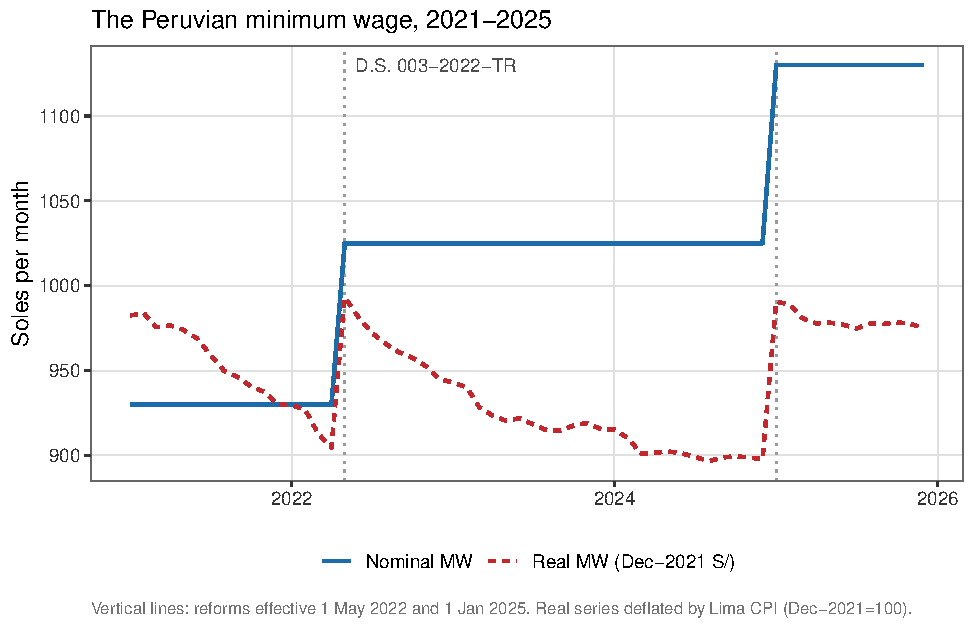
\includegraphics[width=0.82\textwidth]{fig1_minimum_wage.pdf}
\caption{The nominal and real Peruvian minimum wage, 2021--2025. The real series is
deflated by the Lima consumer price index (December 2021 = 100). Vertical dotted
lines mark the reforms effective 1 May 2022 (Supreme Decree 003-2022-TR) and 1
January 2025 (Supreme Decree 006-2024-TR).}
\label{fig:mw}
\end{figure}

\section{Related literature}\label{sec:literature}

My paper connects three strands of research: the theory and evidence on minimum wage employment effects, the evidence for developing countries with large informal sectors, and the specific literature on Peru.

\paragraph{Theory and the canonical evidence.} The competitive model predicts that a binding wage floor reduces employment among low-productivity workers, with an effect whose size depends on labor demand elasticities and on the fraction of workers bound by the floor \citep{brown_1999}. Models with employer wage-setting power deliver different predictions: under monopsony a moderate minimum wage can raise employment, and it typically compresses the lower tail of the wage distribution \citep{manning_2003}. The empirical literature has moved from a presumption of sizable disemployment toward a consensus of small effects on the margin studied. The case study of \citet{card_krueger_1994} and the broader synthesis in \citet{card_krueger_1995} found little evidence of job loss from the New Jersey reform, and the border-discontinuity design of \citet{dube_lester_reich_2010} and the bunching approach of \citet{cengiz_2019} likewise find that recent United States increases raised wages at the bottom with limited employment effects; \citet{manning_2021} reads the accumulated evidence as an ``elusive'' employment effect, while \citet{neumark_wascher_2007} offer the skeptical reading. \citet{harasztosi_lindner_2019} show that a large Hungarian increase was absorbed mostly through prices rather than employment. Closest to my mechanism, \citet{dustmann_2022} show that the German minimum wage operated through \emph{reallocation}, moving workers across establishments, rather than through employment losses, and \citet{engbom_moser_2022} document how a rising Brazilian minimum compressed the formal wage distribution; \citet{derenoncourt_montialoux_2021} trace distributional consequences of coverage extensions in the United States. A recurring theme, which I build on directly, is that effects should be measured where the minimum ``bites.'' \citet{card_1992} uses regional variation in the fraction of workers affected, \citet{clemens_wither_2019} follow workers whose wages sat below a rising federal floor, \citet{lee_1999} uses the gap between the minimum and the median wage, and \citet{machin_manning_rahman_2003} exploit a low-wage sector in which the introduction of the United Kingdom minimum was especially binding. My education-based design is an application of the same logic to a single national reform.

\paragraph{Developing countries and informality.} In economies with large informal sectors the minimum wage interacts with the boundary between covered and uncovered work, and two opposing forces appear repeatedly. A ``lighthouse'' effect can raise wages even in the informal sector, where the minimum serves as a norm or reference \citep{lemos_2009, bosch_manacorda_2010, maloney_nunez_2004}, while a reallocation effect can push workers out of formal employment and into informal or self-employed arrangements \citep{ham_2018_honduras}; \citet{ulyssea_2018} provides the modern equilibrium framework in which regulation shifts firms and workers across the formality boundary. The Latin American evidence spans this range. Early work on Mexico and Colombia found disemployment where the floor was high relative to wages \citep{bell_1997}, and \citet{gindling_terrell_2007} show for Costa Rica that legal floors move wages only in the covered sector. Studies of Brazil find wage compression with small employment effects and evidence of spillovers into the informal sector \citep{lemos_2009, lemos_2004}; \citet{jales_2018} estimates, with a density approach, that the Brazilian minimum moves a substantial share of workers into informality. Work on Ecuador finds positive wage effects concentrated among low-income workers \citep{wong_2019_ecuador}, and \citet{arango_2022_colombia} collect the recent Colombian evidence. The Honduran case is the clearest counterexample to the lighthouse view: \citet{ham_2018_honduras} documents that a high minimum wage reduced covered employment and shifted workers toward informality, with no reduction in poverty. For Uruguay, \citet{katzkowicz_2021_uruguay} use a density-discontinuity approach in the domestic-work sector to show that effects concentrate among the least skilled. The common methodological thread is the use of exposure or bite measures, either geographic Kaitz indices or fraction-affected shares, and a careful accounting of the informal margin, both of which I adopt.

\paragraph{Peru.} The domestic literature is thin and, until recently, dated; the margin I emphasize has, however, begun to attract attention, with \citet{corcuera_2024} studying the response of informal self-employment to Peruvian minimum wage increases in earlier data. Early studies of the reforms of the early 2000s find small and often statistically weak effects. \citet{jaramillo_lopez_2006} analyze the 2003 increase using short quarterly panels for metropolitan Lima and conclude that the reform was largely innocuous, with negative employment-retention effects concentrated near the floor and evidence of displacement from the formal to the informal sector. \citet{cespedes_2005} estimates a weakly significant employment elasticity of about $-0.13$ and shows that the RMV Granger-causes formal wages, an early statement of the lighthouse view for Peru. The most credible modern study is \citet{jimenez_2023}, who evaluates the 2016 reform using a difference-in-differences design with a department-level treatment dose, defined as the pre-reform share of formal workers earning between the old and new minimum. That study finds no disemployment, a rise in formality of 2.5 to 2.8 percentage points, and wage gains of 4.1 to 5.4 percent, and it interprets the pattern through employer market power, of the kind \citet{amodio_deroux_2021} document directly in Colombian manufacturing plants. My paper differs from this precedent in three respects that I make explicit. I study a later reform and the post-pandemic period; I define exposure at the worker level through education rather than at the department level; and I find a different pattern of adjustment, with no wage gain and a decline rather than an increase in formality. I return to the reconciliation of these findings in Section~\ref{sec:discussion}. As \citet{jimenez_2023} emphasizes, the binding constraint for any Peruvian design is the absence of sub-national variation in the nominal minimum, which forces the researcher to manufacture differential exposure; my contribution is to do so through the education dimension and to trace the consequences for the formal and informal margins.

\paragraph{Econometrics of difference-in-differences.} Methodologically I rely on the modern difference-in-differences literature. Because my reform occurs at a single date, the recent concerns about negative weighting and forbidden comparisons under staggered adoption \citep{goodmanbacon_2021, dechaisemartin_2020, sun_abraham_2021, callaway_santanna_2021} do not bind: with a common treatment date the two-way fixed-effects estimator and its event-study analog are unbiased for a convex average of group-time effects \citep{roth_2023_trending, baker_larcker_wang_2022}. I nonetheless use the doubly robust estimator of \citet{santanna_zhao_2020} as a building block, and I take the threat to identification, namely differential trends by skill, seriously through the sensitivity analysis of \citet{rambachan_roth_2023}. For inference with few clusters I follow \citet{bertrand_2004}, \citet{cameron_2008_bootstrap}, and \citet{pustejovsky_tipton_2018}; selection into the wage sample is bounded with the trimming approach of \citet{lee_2009}. Distributional effects are estimated with the unconditional quantile method of \citet{firpo_fortin_lemieux_2009}.

\section{Data and measurement}\label{sec:data}

\subsection{The ENAHO quarterly employment modules}

I use the public-use quarterly files of the Encuesta Nacional de Hogares (ENAHO), the national household survey conducted by Peru's Instituto Nacional de Estadística e Informática (INEI). ENAHO is a nationally representative, stratified, multi-stage survey with continuous fieldwork; the quarterly employment and income module (module 500) records detailed labor market information for each household member of working age. I pool the sixteen quarters from the first quarter of 2021 through the fourth quarter of 2024, about 347,000 person-quarter records in total, of which roughly 278,000 working-age observations with non-missing education enter the baseline estimation sample (the partially treated transition quarter 2022Q2 is excluded; see Section~\ref{sec:strategy}). I add the four quarters of 2025 for the out-of-sample validation exercise. All statistics use the module's sampling weights; the treatment of standard errors is discussed in Section~\ref{sec:strategy}.

For the worker-level transition analysis of Section~\ref{sec:transitions} I complement the quarterly cross-sections with the ENAHO Panel 2020--2024, the survey's linked component, which re-interviews the same dwellings annually and identifies the same persons across years. Consecutive-year pairs link 23,000 to 24,000 persons, and INEI publishes dedicated panel expansion factors that adjust for attrition and non-response. Appendix~A documents the source files, the linkage indicators, and the construction of the transition states.

The quarterly frequency I exploit is part of the survey design rather than an ad hoc partition of an annual file. ENAHO's technical documentation lists two official inference levels for the integrated sample: annual (national, urban and rural, each of the 24 departments, natural regions, and metropolitan Lima) and \emph{quarterly} (national, urban national, and rural national), so national quarterly estimation is sanctioned by the sampling design itself. Moreover, in the non-panel sample the same conglomerates are visited in the same month every year, with different dwellings drawn within them, so the geographic and seasonal composition of each quarter is held fixed across years; in my files, 70 percent of primary sampling units overlap between the same quarter of consecutive years, against 5 percent between different quarters. Each quarter contains close to one fourth of the annual sample (about 1{,}340 conglomerates and 21{,}000--22{,}000 working-age records) with stable composition across quarters. Department-level inference, by contrast, is annual only; accordingly, I use department-by-quarter variation solely through fixed effects and collapsed cells, and I measure the regional bite by pooling the five pre-reform quarters, which approaches the annual level at which departmental estimates are representative.

I restrict the sample to individuals of working age, defined as ages 14 to 65,\footnote{Fourteen is the minimum legal working age in Peru; 65 is the conventional upper bound of the working-age population.} and I drop observations with missing education. My main wage analysis is further restricted to private-sector wage earners,\footnote{White- and blue-collar employees and domestic workers, ENAHO occupational-category variable \texttt{p507} equal to 3, 4, or 6; domestic workers have been entitled to the minimum wage since Law 31047 (2020). Employers, own-account workers, and unpaid family workers are treated as separate categories, and public-sector workers are excluded from job-level outcomes because their pay is set by separate scales.} for whom the minimum wage is the relevant statutory floor, while the employment and participation outcomes are defined over the working-age population and the formality and self-employment outcomes over employed private-sector workers.

\subsection{Education and the definition of skill groups}

The treatment and comparison groups are defined by educational attainment, recorded in ENAHO variable \texttt{p301a}, the highest level of schooling completed. I validated the coding of this variable against the weighted distribution of attainment in the data; it corresponds to the standard INEI classification, ranging from no schooling through postgraduate study. I define \emph{low-skilled} workers as those with at most complete secondary schooling (no education, initial, primary, or secondary), and \emph{high-skilled} workers as those with any tertiary schooling (non-university higher, university, or postgraduate). I exclude the small residual category of special education, which is not ordered on the skill dimension, and observations with missing education.

This partition has three attractive features. First, it is a bright line in the Peruvian labor market: completion of tertiary schooling is the main credential that separates workers who compete for jobs paying near the minimum wage from those who do not. Second, it splits the working-age population into groups of comparable size, roughly two thirds low-skilled and one third high-skilled, which gives adequate statistical power on both sides. Third, and most important for identification, the two groups differ sharply in their exposure to the minimum wage. As Table~\ref{tab:desc} shows, in the pre-reform period the median monthly wage of a low-skilled dependent employee is close to the statutory floor, whereas the median high-skilled employee earns well above it. The classification follows a long line of work that treats education as a primary determinant of where the minimum wage bites \citep{lemos_2009, katzkowicz_2021_uruguay}.

\subsection{Outcome variables}

The outcomes fall into three groups. On \emph{pay}, ENAHO records wage earners' pay per pay period together with its frequency; because over half of low-education wage earners are paid daily, weekly, or fortnightly, against fifteen percent of high-education wage earners, I convert all payments to monthly equivalents using the frequency variable before any comparison across groups (Appendix~\ref{app:data} details the conversion, which matches INEI's own annualization). The real hourly wage divides this monthly-equivalent labor income by monthly hours, deflated by the Lima consumer price index at the month the income refers to, in December 2021 soles, and winsorized at the first and last half-percentiles; real monthly earnings is the same numerator without the hours adjustment. On \emph{quantities}, employment and labor force participation are indicators defined over the working-age population, and weekly hours is hours worked in the main occupation. On \emph{composition}, formal employment and self-employment are defined among employed private-sector workers, and an indicator for being paid below the statutory minimum in force in the income reference month is defined among private wage earners; the last is a direct measure of the bite of and compliance with the policy.

A measurement issue arises for informality. INEI's official informal-employment indicator, \texttt{ocupinf}, is present in the 2021 through 2023 files but is not released in the 2024 and 2025 files. Because my study window extends through 2024, I reconstruct a consistent informality indicator from underlying primitives that are available in every year: pension affiliation, the possession of a formal labor contract, the registration status of the productive unit, and the category of employment. I validate the reconstruction against the official \texttt{ocupinf} in 2021 through 2023, where both are available, and obtain agreement of about 88 percent at the worker level, with an implied informality rate of 74.9 percent against the official 79.1 percent. I use the official indicator wherever it exists and the reconstruction only for 2024 and 2025, and I report a robustness check that restricts the formality analysis to the years covered by the official measure. Full details of the construction are in Appendix~\ref{app:data}.

\subsection{Descriptive statistics}

Table~\ref{tab:desc} reports weighted means of the main variables by skill group in the pre-reform period. The two groups differ in the expected ways. Low-skilled workers are older on average, more likely to be married and rural, and have far lower wages. The employment rate is similar across groups, but the composition of employment differs starkly: low-skilled workers are much more likely to be informal and self-employed, and far more likely to earn below the statutory minimum. Among private wage earners, 57 percent of the low-skilled were paid below the \emph{new} minimum of 1,025 soles on the eve of the reform, against 40 percent of the high-skilled. This is the exposure gap on which my design rests, though the substantial exposure of the comparison group also means the design estimates a relative rather than an absolute effect. The high informality of the low-skilled group, 87 percent against 53 percent for the high-skilled, is central to interpreting the results: for most low-skilled workers the statutory floor is not directly enforced, so the margin along which the labor market can adjust is the allocation of workers across formal and informal arrangements rather than the level of pay within formal jobs.

\begin{table}[H]\centering
\caption{Descriptive statistics by skill group, pre-reform period}\label{tab:desc}
\begin{threeparttable}
\begin{tabular}{lccc}
\toprule
 & Low-skilled & High-skilled & Difference \\
 & ($\le$ sec. complete) & ($\ge$ higher) & \\
\midrule
Age & 35.92 & 34.65 & 1.27 \\
Female & 0.50 & 0.50 & 0.00 \\
Urban & 0.76 & 0.93 & -0.17 \\
Married & 0.53 & 0.41 & 0.12 \\
Years of education & 8.57 & 14.47 & -5.90 \\
Labour force participation & 0.73 & 0.80 & -0.07 \\
Employed & 0.69 & 0.73 & -0.04 \\
Wage employee (incl. domestic) & 0.29 & 0.48 & -0.19 \\
Self-employed & 0.39 & 0.24 & 0.15 \\
Formal (if employed) & 0.13 & 0.47 & -0.34 \\
Informal (if employed) & 0.87 & 0.53 & 0.34 \\
Weekly hours (if employed) & 39.74 & 41.44 & -1.70 \\
Real hourly wage (S/) & 5.74 & 9.08 & -3.34 \\
Real monthly earnings (S/) & 904.30 & 1,755.12 & -850.82 \\
Below MW (wage earners) & 0.43 & 0.19 & 0.24 \\
\midrule
Observations & 65,954 & 27,278 & \\
\bottomrule
\end{tabular}
\begin{tablenotes}\footnotesize
\item Notes: Weighted means using ENAHO survey weights, working-age individuals (14--65) in the pre-reform quarters (2021Q1--2022Q1). Low-skilled: education at most complete secondary (\texttt{p301a}$\le$6). High-skilled: any tertiary education (\texttt{p301a}$\ge$7). Wage-earner variables (hourly wage, below MW) are conditional on being a private-sector wage earner (employees and domestic workers, monthly-equivalent earnings); hours and formality are conditional on employment. Observation counts are unweighted. The below-MW row uses the statutory floor in force in the income reference month (930 soles throughout the pre-reform window); the exposure shares relative to the NEW floor (57 vs.\ 40 percent) discussed in the text use 1{,}025 soles.
\end{tablenotes}
\end{threeparttable}\end{table}


Figure~\ref{fig:trends} plots the weighted quarterly means of the main outcomes by skill group over the study window, with the reform marked. The raw series already hint at the results that follow: the wage series of the two groups move in parallel throughout, while the formality and self-employment series begin to diverge around the reform. The figure also makes visible a fact that matters for the analysis: in the employment panel it is the \emph{high}-education series that swings, rebounding sharply through 2021 and oscillating thereafter, while the low-education series is comparatively flat, so any employment ``effect'' in the education contrast is driven largely by movements of the comparison group; this is part of why Section~\ref{sec:results} declines to interpret that margin causally. These are unconditional means; the regression analysis that follows adjusts for composition and seasonality.

\begin{figure}[!t]
\centering
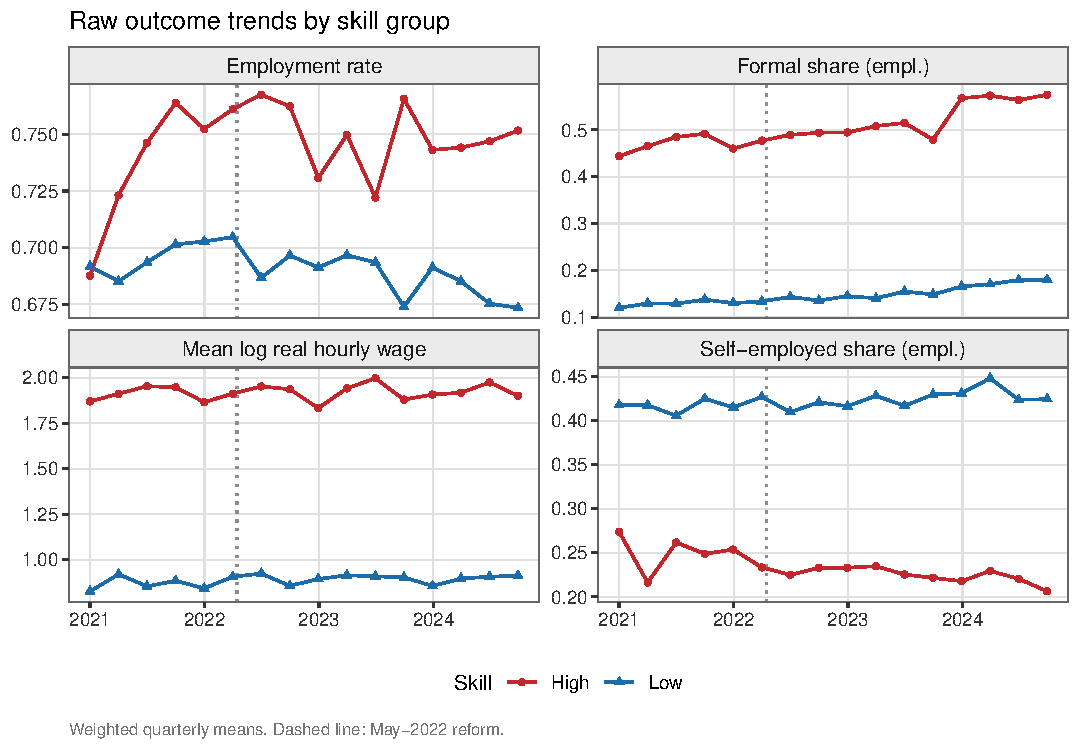
\includegraphics[width=0.95\textwidth]{fig2_raw_trends.pdf}
\caption{Raw outcome trends by skill group, 2021--2024. Weighted quarterly means for low- and high-skilled workers. The dashed vertical line marks the May 2022 reform.}
\label{fig:trends}
\end{figure}

Figure~\ref{fig:bite} displays the regional variation in the bite of the minimum wage, measured by the Kaitz index, the ratio of the new minimum to the pre-reform median monthly-equivalent wage of private wage earners in each department. The index ranges from about 0.79 in Ica to about 1.97 in Huánuco, and it exceeds one in eighteen of the twenty-five departments, so that in much of the country the new minimum exceeds the median wage. This variation is predetermined with respect to the reform and provides the basis for the triple-difference and continuous-intensity checks in Section~\ref{sec:robustness}.

\begin{figure}[!t]
\centering
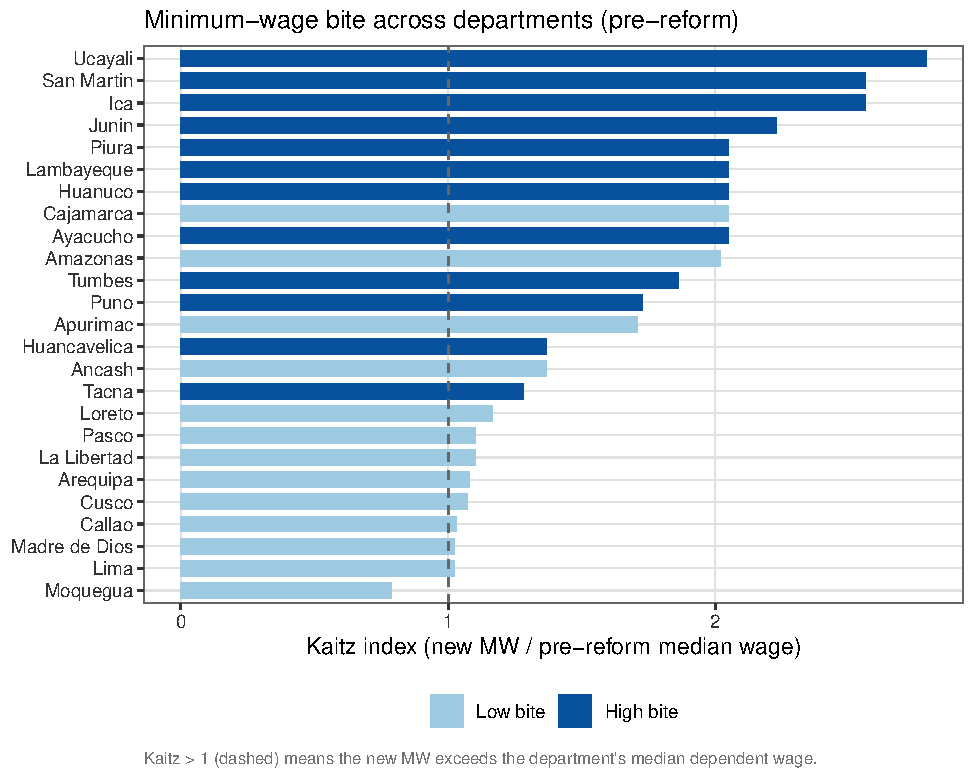
\includegraphics[width=0.72\textwidth]{fig3_regional_bite.pdf}
\caption{Regional variation in the bite of the minimum wage. The Kaitz index is the ratio of the new minimum wage (1,025 soles) to the department's median monthly-equivalent wage of private wage earners in the pre-reform quarters. Departments above the dashed line have a median wage below the new minimum.}
\label{fig:bite}
\end{figure}

\section{Empirical strategy}\label{sec:strategy}

\subsection{Potential outcomes and the estimand}

Let $i$ index individuals, $g\in\{\Low,\mathrm{High}\}$ their skill group, and $t$ the quarter. The reform becomes effective in the second quarter of 2022, which I denote $t^{\ast}$;\footnote{Because the reform took effect on 1 May, the second quarter of 2022 contains one pre-reform and two post-reform months, and reported incomes refer to the month before the interview, so even May interviews report pre-reform (April) earnings. I therefore exclude 2022Q2 from the baseline as a partially treated transition quarter and restore it in a robustness check; the first post-reform quarter in the baseline is 2022Q3.} define the post-reform indicator $\Post_t=\mathbf{1}\{t\ge t^{\ast}\}$ and the treatment indicator $\Low_i=\mathbf{1}\{g_i=\Low\}$. Following the potential-outcomes framework, let $Y_{it}(1)$ and $Y_{it}(0)$ denote the outcome of individual $i$ in quarter $t$ with and without the reform being in force. The parameter of interest is the average effect of the reform on the low-skilled, relative to the counterfactual in which they had experienced the same evolution as the high-skilled,
\begin{equation}
\mathrm{ATT} \;=\; \mathbb{E}\!\left[\,Y_{it}(1)-Y_{it}(0)\;\middle|\;\Low_i=1,\;t\ge t^{\ast}\right].
\end{equation}
The data are repeated cross-sections rather than a panel, so the object is identified from comparisons of group means over time rather than from within-person changes.

Because Peru's minimum wage is national and changes on a single date, there is no variation in treatment \emph{timing}; every worker is exposed to the same policy at the same moment. Identification instead rests on variation in the \emph{intensity} of exposure across skill groups. The design is therefore a canonical two-group difference-in-differences with many periods, not a staggered-adoption design. This distinction matters for the choice of estimator. The recent econometric literature has shown that the two-way fixed-effects estimator can be badly biased when treatment timing is staggered and effects are heterogeneous \citep{goodmanbacon_2021, dechaisemartin_2020, sun_abraham_2021, callaway_santanna_2021}. With a common treatment date, however, these problems do not arise: the two-way fixed-effects estimator and its event-study analog recover a convex, properly weighted average of treatment effects \citep{roth_2023_trending, baker_larcker_wang_2022}. I nonetheless report the doubly robust estimator of \citet{santanna_zhao_2020} as a complementary building block.

\subsection{Estimating equations}

My baseline specification is the two-way fixed-effects difference-in-differences model
\begin{equation}
Y_{idt} \;=\; \beta\,(\Low_i\times\Post_t) \;+\; \gamma\,\Low_i \;+\; \lambda_t \;+\; \mu_d
\;+\; X_{it}'\theta \;+\; \varepsilon_{idt},
\label{eq:twfe}
\end{equation}
where $d$ denotes the department, $\lambda_t$ are quarter fixed effects, $\mu_d$ are department fixed effects, and $X_{it}$ is a vector of controls comprising age, its square, sex, an urban indicator, marital status, and years of education (which captures variation in attainment within skill groups). The coefficient $\beta$ is the difference-in-differences estimate. The quarter fixed effects absorb any shock common to both skill groups in a given quarter, including aggregate inflation, so that estimates in logs are invariant to whether wages are expressed in nominal or in nationally deflated real terms. Observations are weighted by the survey weights, and standard errors are clustered by department.

To trace the dynamics of the effect and to test the identifying assumption, I estimate the dynamic event-study specification
\begin{equation}
Y_{idt} \;=\; \sum_{k\neq -1}\beta_k\,\bigl(\Low_i\times\mathbf{1}\{t-t^{\ast}=k\}\bigr)
\;+\; \gamma\,\Low_i \;+\; \lambda_t \;+\; \mu_d \;+\; X_{it}'\theta \;+\; \varepsilon_{idt},
\label{eq:event}
\end{equation}
where $k$ indexes quarters relative to the reform and the quarter immediately before the reform ($k=-1$, the first quarter of 2022) is the omitted reference. The coefficients $\beta_k$ for $k<0$ measure differential pre-trends between the skill groups and provide a direct test of parallel trends; the coefficients for $k\ge 0$ trace the path of the effect.

\subsection{Identifying assumptions and threats}

Identification of the ATT from equation~\eqref{eq:twfe} requires that, absent the reform, the outcomes of low- and high-skilled workers would have followed parallel paths, conditional on the controls and fixed effects. Three threats deserve attention.

First, \emph{differential trends}. Education is correlated with sector, region, and formality, and the two skill groups could have been on diverging paths for reasons unrelated to the minimum wage. I assess this directly through the pre-reform event-study coefficients and a joint test of their equality to zero, and I probe robustness to department-specific linear trends. Because my window opens in the depth of the pandemic recovery, when the employment of low- and high-skilled workers rebounded at different rates, I pay particular attention to the first quarter of 2021 and report specifications that drop it.

Second, \emph{sensitivity to residual violations}. Even when pre-trends are statistically flat, they need not be exactly zero. I therefore report the sensitivity analysis of \citet{rambachan_roth_2023}, which asks how large a post-reform violation of parallel trends, relative to the largest violation observed before the reform, would be needed to overturn each conclusion.

Third, \emph{spillovers and general equilibrium}. If the reform displaces low-skilled workers into the informal sector, it may indirectly depress wages there, and if high-skilled workers are imperfect substitutes their outcomes could also move, contaminating the comparison group. I cannot rule this out, and I interpret the estimates as relative effects. The comparison group is not entirely unexposed: 40 percent of high-skilled private wage earners were paid below the new floor before the reform, against 57 percent of the low-skilled. To first order this imperfect exposure attenuates the estimates toward zero (the design identifies the effect of the seventeen-point exposure \emph{gap}, so it understates the effect on the fully exposed), but I acknowledge that it also makes the estimates relative objects rather than absolute ones. For this reason I complement the education contrast with a continuous regional-exposure design that does not rely on the comparison group at all (Section~\ref{sec:robustness}).

\subsection{Inference}

The treatment is assigned at a coarse level, the skill group, which raises the standard concern that conventional standard errors overstate precision \citep{bertrand_2004}. I address this in several complementary ways. My baseline clusters by department,\footnote{The 25 clusters are Peru's 24 departments plus the Constitutional Province of Callao. With few clusters, conventional cluster-robust standard errors can understate uncertainty, which motivates the additional corrections below.} which allows arbitrary within-department correlation across individuals and quarters; I report an alternative that clusters by department and skill group; and I apply the bias-reduced CR2 small-sample correction of \citet{pustejovsky_tipton_2018} to department-level collapsed cells, where it is computationally feasible. Because these corrections may still be optimistic with a two-group design, I complement them with randomization inference at the department level, permuting the regional bite of the minimum wage across departments to construct an exact null distribution for the exposure-intensity design.

\section{Main results}\label{sec:results}

\subsection{The reallocation of low-skilled employment}

The central result of the paper is that the 2022 reform shifted the composition of low-skilled employment away from formal wage work and toward self-employment, without raising the pay of the workers it targeted. I present the compositional evidence first, then the first-stage evidence on where the floor binds, and the wage evidence third.

The estimated effect on the probability of formal employment among employed private-sector workers is $-0.046$ (column 1 of Table~\ref{tab:main}), a decline of 4.6 percentage points for low-skilled relative to high-skilled workers, about a fifth of the group's 23 percent baseline formality rate. The implied semi-elasticity is large (about $-2$ with respect to the 10.2 percent increase, column 4 of Table~\ref{tab:main}), but this reflects how small the formal base is for this group rather than an implausibly elastic response. The estimate is precisely estimated under department clustering, and the pre-trend test does not reject parallel trends ($p=0.15$); Section~\ref{sec:robustness} takes the residual-drift concern seriously and shows that drift-adjusted magnitudes remain economically large and coincide with the synthetic-DiD estimate. The event study in Figure~\ref{fig:event} shows the relative formality of the low-skilled dropping immediately after the reform, by around four percentage points within a year, and persisting. Mirroring this, the probability of self-employment rises by 3.6 percentage points. The self-employment series, unlike formality, does show a rejected pre-trend test ($p=0.003$), driven by one elevated quarter in mid-2021, so I lean on the formality margin as the cleaner of the two and treat the self-employment estimate as its corroborating mirror image. Weekly hours in the main occupation rise modestly and full-time status falls slightly, consistent with a shift toward own-account work, where hours are less standardized.

Two independent pieces of evidence support a causal reading of this reallocation. First, it scales with exposure: as Section~\ref{sec:heterogeneity} shows, the formality decline and the self-employment rise are both larger in the departments where the new floor cuts deeper into the pre-reform wage distribution. Second, a continuous-exposure design in the spirit of \citet{card_1992}, which discards the education contrast altogether and relates outcomes to the standardized pre-reform regional Kaitz index, yields the same picture: a one-standard-deviation higher regional bite is associated with a 1.8 percentage-point larger decline in formality and a 1.0 point larger rise in self-employment after the reform, estimates that survive design-based randomization inference at the department level (Section~\ref{sec:robustness}). Taken together these results describe a reallocation of low-skilled workers away from formal salaried jobs and toward own-account work, the classic informalization margin emphasized by \citet{jaramillo_lopez_2006} for Peru and by \citet{ham_2018_honduras} for Honduras.

\input{../../tables/tab_main_did}

\subsection{The first stage: where the floor is enforced, it binds}

Where does the statutory floor actually bind? Pinning this down first helps to interpret the pay results that follow. Table~\ref{tab:firststage} and Figure~\ref{fig:bunching} examine the earnings distribution of \emph{formal} private wage earners, the segment where enforcement is concentrated, in symmetric three-quarter windows around the reform. Before the reform, 14 percent of low-skilled formal wage earners are paid within 2.5 percent of the old floor of 930 soles, a visible spike in the manner of \citet{cengiz_2019} and \citet{engbom_moser_2022}. After the reform the spike migrates essentially completely: the mass at 930 collapses to under 2 percent and an almost identical spike, 14 percent, appears at the new floor of 1,025. Formal-sector employers, in other words, complied with the new minimum.

The compliance response splits exactly along the enforcement boundary. Panel B of Table~\ref{tab:firststage} estimates the DiD for an indicator of pay below 1,025 soles, holding the threshold fixed in all periods. Among formal wage earners the share below the new floor falls by five percentage points for low- relative to high-skilled workers (marginally significant, $p=0.10$); among \emph{informal} wage earners it \emph{rises} by four percentage points ($p=0.002$): informal pay drifted further below a floor that does not apply in practice. The two responses offset in the pooled fixed-threshold estimate (last row of Panel B), which is also why the statutory below-minimum indicator of Table~\ref{tab:main} shows no change. Together with the reallocation results, this evidence describes a coherent two-sector adjustment: the floor binds and is honored inside the formal sector, formal employment of the affected group contracts, and the displaced margin reappears as self-employment and informal work whose pay the floor does not reach.

\begin{figure}[!t]
\centering
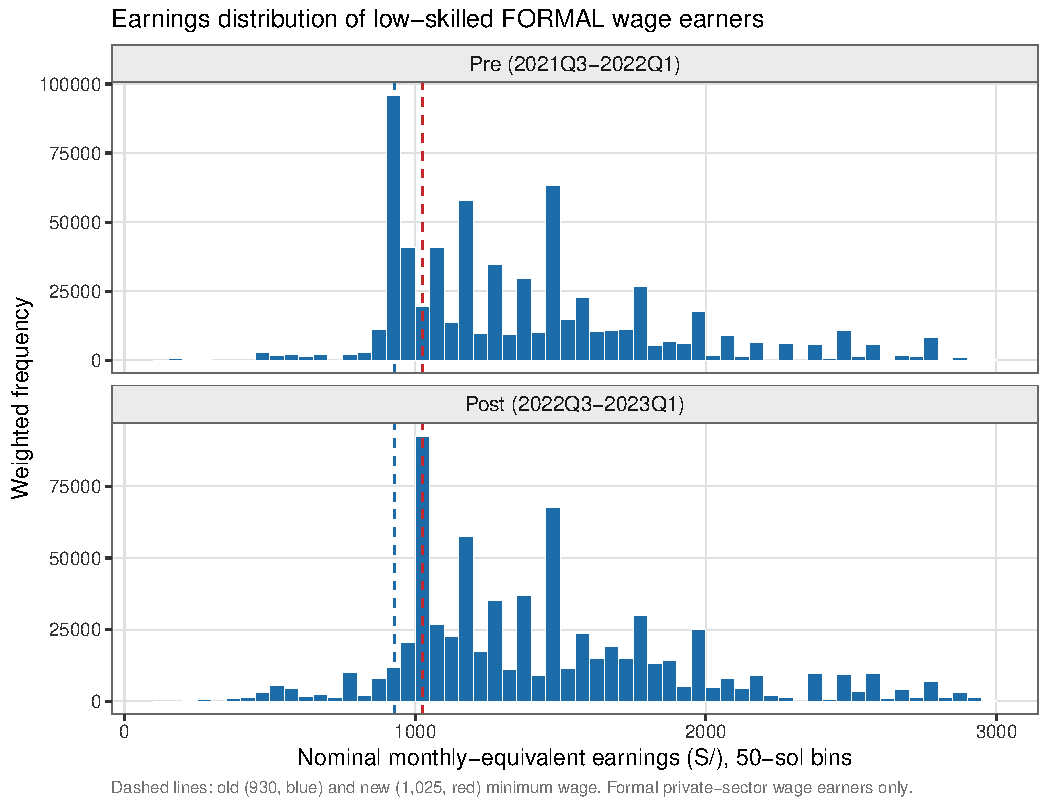
\includegraphics[width=0.8\textwidth]{fig10_bunching.pdf}
\caption{Spike migration at the wage floor among low-skilled formal private wage earners. Weighted histograms of nominal monthly-equivalent earnings (50-sol bins) in symmetric three-quarter windows before (2021Q3--2022Q1) and after (2022Q3--2023Q1) the reform. Dashed lines mark the old (930) and new (1,025) minimum wage.}
\label{fig:bunching}
\end{figure}

\input{../../tables/tab_firststage}

\subsection{The wage response}

If covered employers complied with the new floor, did the pay of the low-skilled group rise as a whole? On average it did not. The coefficient on the interaction of the low-skill indicator with the post-reform indicator is $-0.021$ for the log real hourly wage, with a standard error of $0.012$: negative, marginally insignificant, and inconsistent with the reform having lifted relative pay. The estimate for log monthly earnings is similarly null. I am deliberately careful about how much this regression can bound, for a transparent reason reported in column (3) of Table~\ref{tab:main}: the joint pre-trend test for the hourly wage rejects ($p=0.001$), driven by a single positive spike in 2021Q2 ($k=-4$) rather than by a systematic trend. Once violations of parallel trends are allowed, the education contrast cannot pin the wage effect tightly in either direction: under the relative-magnitudes restriction of \citet{rambachan_roth_2023} the robust interval at exact parallel trends reaches $+2.9$ percent, and under linear extrapolation of the (gently declining) pre-trend even larger positive values are admissible. I therefore do not rest the no-lift conclusion on the average wage regression. It rests on the two pieces of pay evidence whose diagnostics are clean and which do not depend on the education pre-trend.

First, the share of wage earners paid below the statutory floor, which was 35 percent among low-skilled wage earners at baseline, does not fall after the reform (the estimate is $-0.006$ with $p=0.45$, and its pre-trends are flat, $p=0.13$). If firms had complied with the new floor for the marginal worker, this share would have dropped mechanically. Second, the earnings distribution in Figure~\ref{fig:dist} shows visible mass near the old minimum before the reform but no appreciable migration of that mass toward the new floor afterward, reflecting the pervasive non-compliance documented in Section~\ref{sec:data}; the unconditional-quantile estimates of Section~\ref{sec:heterogeneity} likewise show no gain at any decile, including the bottom ones where an enforced floor must compress the distribution.

The doubly robust estimator of \citet{santanna_zhao_2020} in column (2) of Table~\ref{tab:main} deserves a candid reading rather than a footnote. It collapses the sixteen quarters to a single pre- and post-reform comparison and omits department fixed effects, and under department-clustered standard errors it is imprecise for every outcome: the wage estimate is negative ($-0.056$, standard error $0.137$) and the formality estimate is a null ($+0.006$, standard error $0.040$) rather than the two-way fixed-effects $-0.046$. I read this as the familiar cost of discarding the time-series structure \citep{bertrand_2004}: collapsing to two periods and twenty-five clusters leaves little identifying variation, and the resulting confidence intervals contain both zero and effects twice my baseline. It is why I treat the doubly robust column as a conservative complementary check rather than as the preferred estimate, and why the corroboration I lean on instead comes from designs that retain independent variation: the synthetic-DiD estimate on department cells and the continuous regional-exposure design of Section~\ref{sec:robustness}.

That the reform failed to lift wages at the bottom is not surprising in this setting: once inflation is netted out the real value of the floor rose little, most low-skilled workers are informal or self-employed, and enforcement is thin, so the statutory minimum constrains pay for only a minority. The absence of a pay response contrasts with the ``lighthouse'' pattern that \citet{jimenez_2023} finds for the 2016 reform. I take up these mechanisms, and the contrast with earlier reforms, in Section~\ref{sec:discussion}.


\subsection{The level of employment}

The estimated effect on the overall employment rate is $-2.5$ percentage points, which would imply an employment elasticity with respect to the minimum wage of about $-0.35$, more than twice the largest estimates in the earlier Peruvian literature \citep{cespedes_2005}. I do not give this estimate a causal interpretation, for three reasons documented in Section~\ref{sec:robustness}: the employment series carries a clear differential pandemic-recovery pre-trend concentrated in early 2021 (pre-trend $p<0.001$); in-time placebo reforms placed in the pre-period produce ``effects'' of similar magnitude and significance; and, unlike the compositional margins, the employment effect does not scale with regional exposure; if anything it is smaller in high-bite departments. Once 2021Q1 is excluded the point estimate roughly halves, and it does not survive the more conservative inference procedures. I therefore treat the employment-level result as reflecting differential recovery dynamics rather than the minimum wage, and place the interpretive weight on the compositional shift, whose diagnostics are clean.

\subsection{Worker-level transitions: the entry margin}\label{sec:transitions}

The compositional results describe net stocks. To identify the gross flow behind them, I complement the repeated cross-sections with the ENAHO Panel 2020--2024, which re-interviews the same dwellings annually and links persons across years (Section~\ref{sec:data}; construction details in Appendix~A). I stack the four year-to-year pairs from 2020--21 through 2023--24 and classify each pair relative to the reform using the 2022 interview month: pre-reform pairs, reform-window pairs whose base state is measured before May 2022 and whose destination is measured after, and post-reform pairs. Among workers holding a formal private job in the base year, I estimate a stacked difference-in-differences for each destination state, with pair and department fixed effects, individual controls, panel weights that adjust for attrition, and standard errors clustered by department. Table~\ref{tab:transitions} reports the destination shares and the estimates.

Two findings sharpen the mechanism. First, incumbents were not pushed out. Relative to high-educated formal workers, the probability that a low-educated formal worker remains formal \emph{rises} across the reform window (8.3 percentage points, $p=0.055$), and the transition into informal wage work falls ($-4.8$ points, $p=0.076$); transitions into self-employment and non-employment do not move. This is exactly what the first stage implies: within the enforced segment, incumbent workers received the mandated raise and kept their jobs. Second, the entry door closed. Among workers who were informally employed in the base year, the probability that a low-educated worker moves \emph{into} a formal private job falls by 2.1 percentage points ($p=0.011$) in the post-reform pairs, nearly half of the group's 4.5 percent baseline entry rate. The decline in the formality stock documented in Section~\ref{sec:results} is therefore a hiring-margin phenomenon: the reform did not dissolve existing formal matches, it reduced the rate at which new ones were created for low-educated workers. This reading is consistent with the incidence of the compositional effects among the young, women, and secondary earners, the workers most likely to be marginal entrants rather than protected incumbents.

Three caveats bound this evidence. The panel is annual, so I cannot time transitions within the year beyond the interview-month split; the pre-reform benchmark pairs include transitions out of the pandemic year 2020, which were unusually churning; and the formal-base sample is modest (about 7,000 pair-observations), so the retention estimate is only marginally significant. The entry response appears in the post-reform pairs rather than in the immediate reform window, consistent with hiring flows adjusting with a lag. I therefore read the panel evidence as qualitative corroboration of the mechanism, incumbent retention plus reduced formal entry, rather than as precise magnitudes.

\input{../../tables/tab_transitions}

\begin{figure}[!t]
\centering
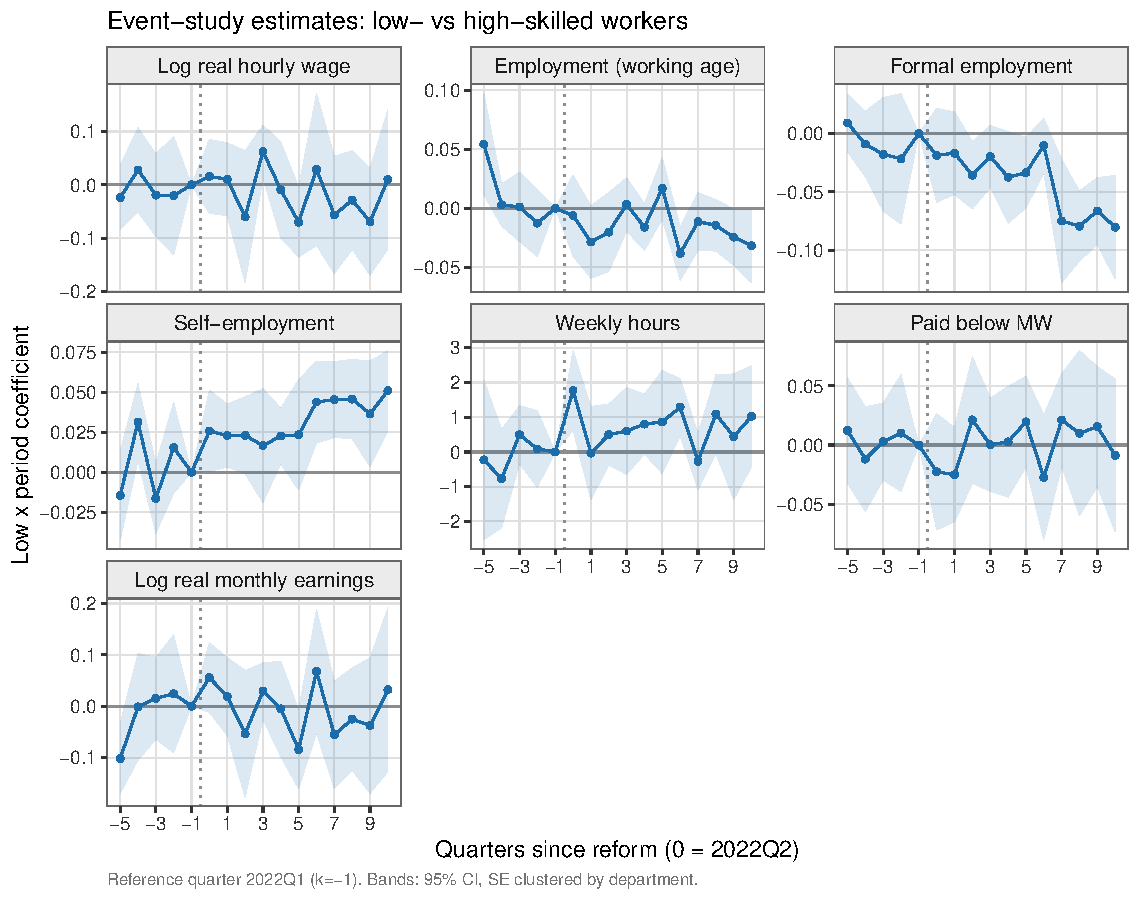
\includegraphics[width=0.98\textwidth]{fig5_event_study.pdf}
\caption{Event-study estimates of the 2022 reform. Each panel plots the coefficients $\beta_k$ on the interaction of the low-skill indicator with quarter indicators from equation~\eqref{eq:event}, relative to the omitted quarter 2022Q1 ($k=-1$). The partially treated transition quarter 2022Q2 ($k=0$) is excluded. Shaded bands are ninety-five percent confidence intervals with standard errors clustered by department.}
\label{fig:event}
\end{figure}

\begin{figure}[!t]
\centering
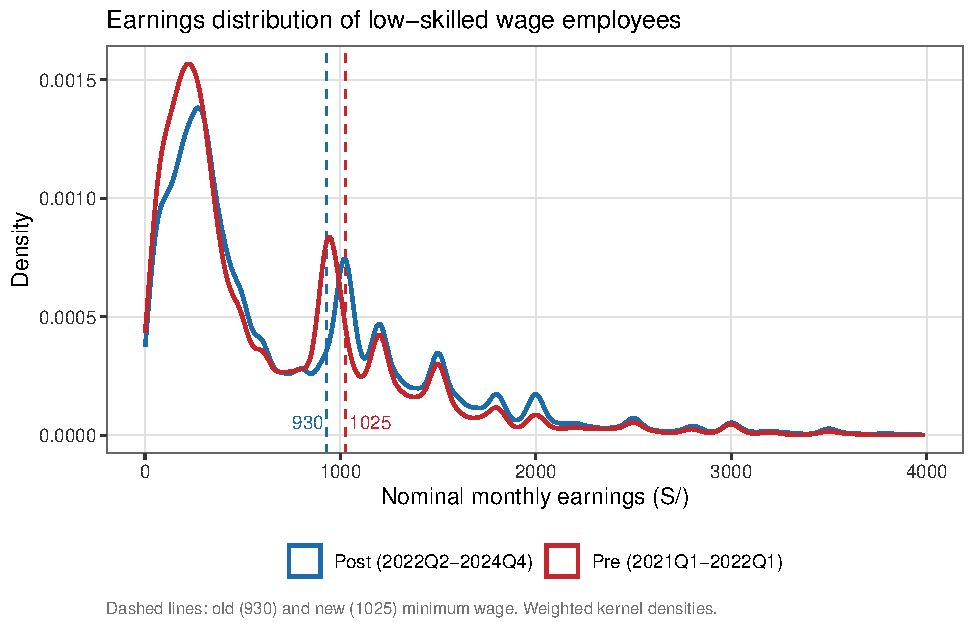
\includegraphics[width=0.72\textwidth]{fig4_wage_distribution.pdf}
\caption{Earnings distribution of low-skilled wage earners, before and after the reform. Weighted kernel densities of nominal monthly-equivalent earnings (private-sector employees and domestic workers), with the old (930) and new (1,025) minimum wage marked by dashed lines.}
\label{fig:dist}
\end{figure}

\section{Robustness and inference}\label{sec:robustness}

This section subjects the main results to a battery of specification, inference, and design checks, and then to an out-of-sample replication. The overall message is that the compositional results, the decline in formality and the rise in self-employment, are the most robust findings, corroborated by an independent continuous-exposure design under randomization inference; the wage evidence consistently shows no pay gain but carries a pre-trend caveat; and the employment-level result fails its diagnostics and should not be read causally.

\subsection{Specification robustness}

Table~\ref{tab:robspec} reports the $\mathrm{Low}\times\mathrm{Post}$ coefficient for the four headline outcomes under ten alternative specifications: dropping the controls, dropping the pandemic quarter of early 2021, adding department-specific linear trends, restricting to prime-age workers, using an alternative education cutoff that removes the categories at the boundary between the two groups, adding occupation and industry fixed effects, clustering by department and skill, restoring the partially treated transition quarter 2022Q2, excluding agriculture (which is covered by the separate agrarian labor regime of Ley 31110 rather than the general minimum wage), and adding public-sector workers back into the job-conditional samples. The formality and self-employment estimates are stable in sign and magnitude throughout, moving within a narrow band. The wage estimate is negative or null in every specification and never significantly positive. The employment estimate, by contrast, attenuates noticeably when the pandemic quarter is dropped or when department-specific trends are included, which reinforces my reluctance to interpret it causally.

\input{../../tables/tab_robustness}

\subsection{Inference}

Because the treatment contrast varies only across two education groups, conventional department clustering does not by itself deliver design-based inference for the $\mathrm{Low}\times\mathrm{Post}$ coefficient, and I therefore report a menu of progressively more demanding procedures. Table~\ref{tab:inference} collects the evidence. Columns (1) through (3) report $p$-values for the baseline effect under department clustering (25 clusters), department-by-skill clustering (50 clusters), and the CR2 small-sample correction of \citet{pustejovsky_tipton_2018} applied to collapsed cells in the spirit of \citet{bertrand_2004}, here at the department$\times$group$\times$period level, which is the finest aggregation at which the CR2 correction is computationally feasible. The formality and self-employment effects remain highly significant under both clustering schemes; under the collapsed-cell CR2 procedure, which is deliberately conservative and low-powered with twenty-five departments, self-employment remains marginally significant and formality does not. The employment effect loses significance under everything beyond simple department clustering. Because a permutation test of the two-group contrast is undefined, design-based randomization inference is conducted for the continuous-exposure design instead, where the assignment being permuted (the regional bite) has twenty-five values: column (4) reports these $p$-values, which belong to the column-(5) estimates, not to the education contrast.\footnote{A wild cluster bootstrap in the spirit of \citet{cameron_2008_bootstrap} is not available for survey-weighted estimation, so the CR2 and randomization procedures play that role here.}

\input{../../tables/tab_inference}

\subsection{Design robustness: bite intensity and triple differences}

My identification rests on differential exposure by education, but the minimum wage also bites differentially across regions, and this provides an independent source of variation that does not rely on the education contrast at all. Column (5) of Table~\ref{tab:inference} reports a continuous-exposure specification in the spirit of \citet{card_1992}, which relates outcomes to the standardized pre-reform department Kaitz index interacted with the post indicator. The results corroborate the skill-based design on the compositional margins: in departments where the minimum wage bites harder, formal employment falls by 1.8 percentage points more per standard deviation of exposure ($p<0.001$; randomization $p<0.001$) and self-employment rises by 1.0 point more ($p=0.02$; randomization $p=0.02$) after the reform. Employment also declines with exposure in this design, though I discount that margin for the reasons above. Wages show no significant response. A triple-difference specification that interacts the skill contrast with an indicator for high-bite departments is not statistically significant for any outcome (Appendix Table~\ref{tab:ddd}), which I read as a lack of power in the coarse binary regional split rather than as evidence against the mechanism, given that the continuous version is informative and that the subgroup estimates in Section~\ref{sec:heterogeneity} move in the expected direction.

Three further design checks qualify this corroboration (Appendix Tables~\ref{tab:expocells} and~\ref{tab:sectorocc}). First, the regional design passes its own leads diagnostic exactly where it matters: joint tests of the pre-reform quarter$\times$exposure interactions do not reject for formality ($p=0.84$), self-employment ($p=0.20$), or wages ($p=0.24$), and reject only for employment ($p=0.002$), consistent with everything else about that margin. Second, in the spirit of full transparency I also estimate finer, cell-level fraction-affected designs \citep{card_1992, clemens_wither_2019}, with exposure measured within department$\times$skill$\times$age cells; these fail their leads diagnostics in both variants: fine-grained exposure is confounded with the cells' heterogeneous pandemic recoveries, and the between-floors variant even flips signs because cells with mass between the two floors are precisely the semi-formal cells that recovered fastest. I therefore treat the department as the credible level for exposure variation and report the cell designs in the appendix rather than suppressing them. Third, the reallocation is broad-based across sectors: the formality decline appears in the covered high-bite sectors, in other private sectors, and in agriculture alike. The agricultural estimate is not a falsification failure, because the agrarian regime's daily remuneration is indexed to the RMV and therefore rose with the reform; Peru leaves no large sector's floor unchanged, which is why coverage contrasts cannot be sharp here. An occupation-level dose response (exposure measured as the pre-reform share of the occupation's wage earners below the new floor) shows larger declines in sub-floor pay and, suggestively, relative wage gains in more-exposed occupations, though occupation is measured post-treatment and I read that panel as descriptive.

As a final design check I estimate synthetic difference-in-differences \citep{arkhangelsky_2021_sdid} on department-by-quarter cells, treating high-bite departments as treated from 2022Q3 and letting the estimator re-weight low-bite departments to reconstruct their pre-reform path (Appendix Table~\ref{tab:sdidpower}). The estimates are directionally consistent with the reallocation (formality falls and self-employment rises, whether the outcome is the low-education mean or the low-minus-high skill gap), with magnitudes about half the TWFE estimates and precision limited by twenty-five aggregate units; the formality decline in low-education means is significant at five percent under the jackknife.

\subsection{Selection and power}

Because the reform moved workers out of the wage-earner sample, the wage DiD conditions on an endogenous population. Appendix Table~\ref{tab:leemde} bounds the resulting bias with the trimming approach of \citet{lee_2009}: the reform reduced low-skilled wage-sample inclusion by 2.1 percentage points (7.6 percent of the baseline rate), and trimming the low$\times$post wage distribution by that fraction from either tail brackets the unconditional 2$\times$2 wage DiD between $-0.10$ and $+0.10$. Selection alone could therefore mask wage effects of up to ten log points in either direction, a candid statement of what the wage evidence can and cannot rule out; the compliance and bunching evidence of Section~\ref{sec:results}, which conditions only on formality status, is not subject to this concern and is where I rest the enforcement conclusion. The same appendix table reports minimum detectable effects: at eighty percent power the design can detect wage effects of 3.4 log points, and effects of 2.1 and 1.7 percentage points on formality and self-employment, both well below the estimated 4.6 and 3.6, so the compositional findings are not an artifact of low statistical power.

The same selection logic applies to the compositional outcomes themselves, which are defined among the employed while the employment margin carries a recovery pre-trend. Appendix Table~\ref{tab:uncond} therefore reports unconditional versions, defined as shares of the working-age population, which involve no conditioning on employment. In the education contrast the unconditional estimates are larger (formal employment $-3.3$ points, self-employment $+1.7$), but they inherit the employment margin's differential pandemic-recovery pre-trend and fail its diagnostic, so I report them for transparency rather than lean on them. The informative result is in the regional design, which does not use the education contrast: unconditional formal employment falls by 1.6 percentage points per standard deviation of exposure (randomization $p<0.001$), so the decline in formal employment is not an artifact of conditioning on a shifting employed population. Unconditional self-employment, by contrast, does not rise with regional exposure; in that design the rise in the self-employment \emph{share} of employment operates through the shrinking employment denominator, and the absolute reallocation into self-employment is a feature of the education contrast specifically. I return to this distinction in Section~\ref{sec:discussion}.

\subsection{Sensitivity to violations of parallel trends}

Even flat pre-trends are estimated with error, so I apply the sensitivity analysis of \citet{rambachan_roth_2023}. Figure~\ref{fig:honest} plots the robust confidence set for the average post-reform effect on employment and formality as I allow the post-reform violation of parallel trends to be as large as a multiple $\bar{M}$ of the largest pre-reform violation. The formality and self-employment effects remain bounded away from zero under exact parallel trends but include zero once violations as large as $\bar{M}=0.1$ are allowed, and the employment effect includes zero even at $\bar{M}=0$. This is the weakest link in the education-based design, and I state it clearly: the compositional results are robust to conventional and to design-based inference, but not to modest violations of parallel trends in the education contrast. Their credibility therefore leans on the two pieces of evidence that do not depend on that contrast: the regional dose-response gradient and the continuous-exposure design with randomization inference. The power calculation of \citet{roth_2022_pretest} quantifies why I do not rely on passed pre-tests alone: a linear violation of parallel trends that my pre-test would detect only half the time would bias the average post-period formality effect by 0.042, nine tenths of the estimated effect (Appendix Table~\ref{tab:sdidpower}, Panel B). Passed pre-tests are reassuring but not conclusive, and I treat them that way throughout the paper.

Timing granularity does not drive the estimates either. Monthly event studies (Figure~\ref{fig:monthly}), which time wage outcomes by the income reference month and employment outcomes by the interview month, show the formality decline appearing immediately after May 2022 and persisting, with a suggestive dip in the weeks around the decree's publication on 3 April; and a quarterly event study that bins the right tail at $k\ge 8$, rather than estimating eleven free lags, leaves the estimates unchanged.\footnote{The full monthly and binned coefficient series are included in the replication package.}

\begin{figure}[!t]
\centering
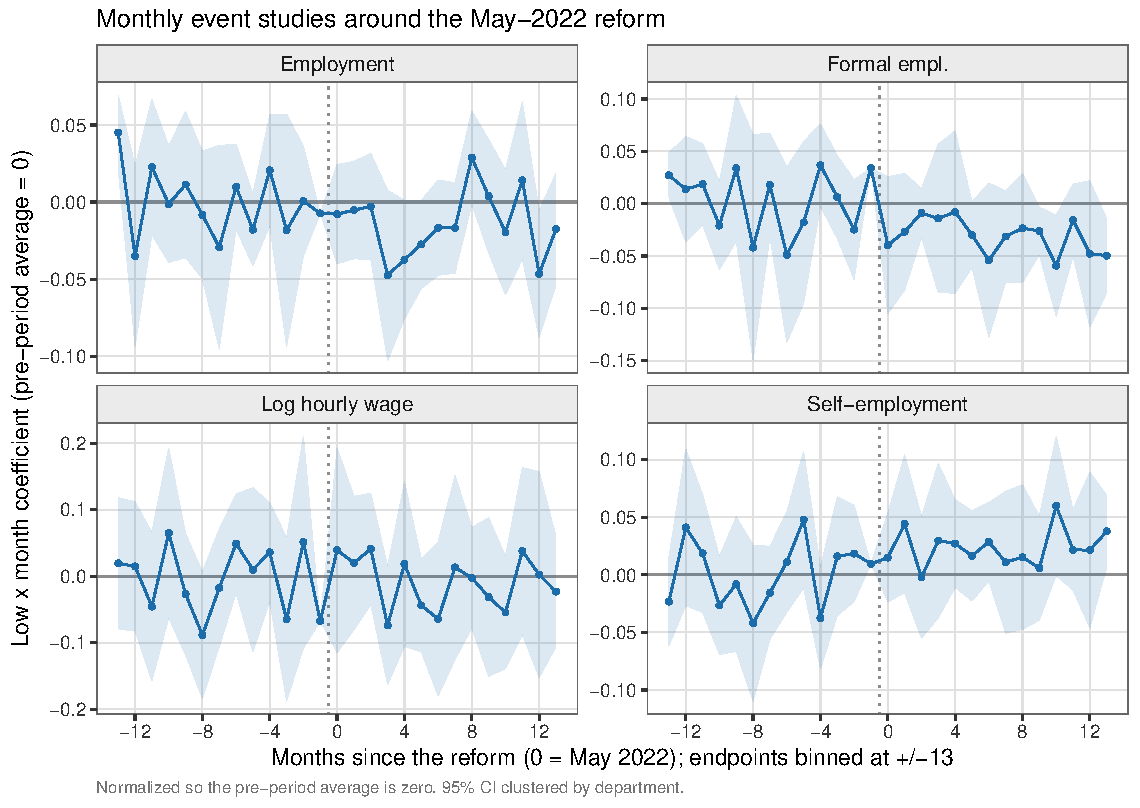
\includegraphics[width=0.98\textwidth]{fig11_monthly_event.pdf}
\caption{Monthly event studies around the May-2022 reform. Wage outcomes are timed by the income reference month and employment outcomes by the interview month; endpoints binned at $\pm$13 months; reference month April 2022. Bands: 95 percent confidence intervals clustered by department.}
\label{fig:monthly}
\end{figure}

\begin{figure}[!t]
\centering
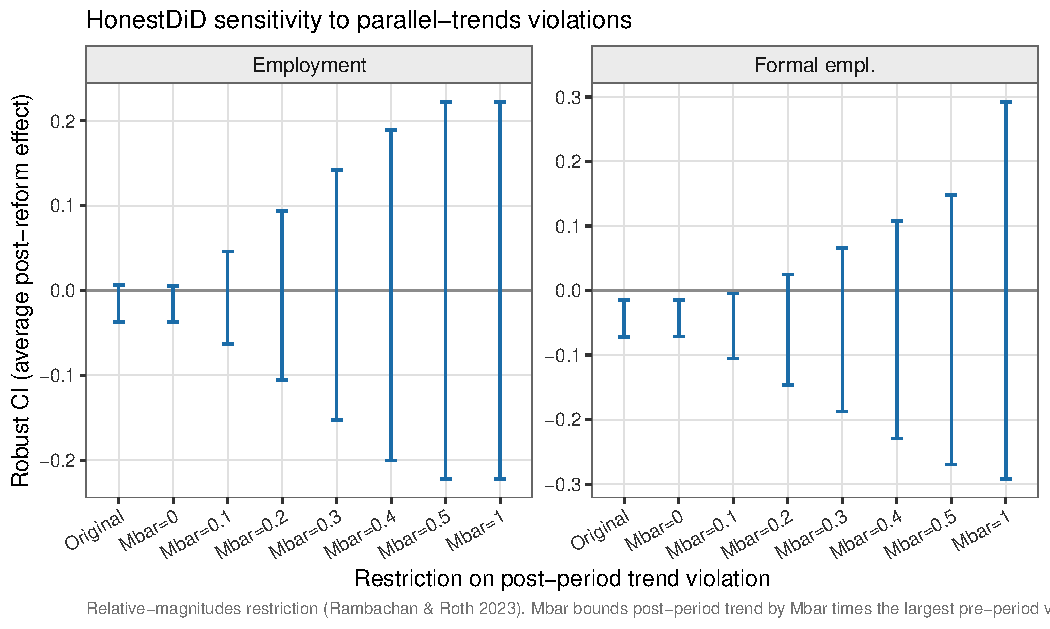
\includegraphics[width=0.8\textwidth]{fig7_honestdid.pdf}
\caption{Sensitivity to violations of parallel trends \citep{rambachan_roth_2023}. Robust confidence sets for the average post-reform effect under the relative-magnitudes restriction, which bounds the post-reform trend violation by $\bar{M}$ times the largest pre-reform violation.}
\label{fig:honest}
\end{figure}

\subsection{Placebo reforms and leave-one-out}

I assign fake reforms to each interior quarter of the pre-reform window and re-estimate the DiD using only pre-reform data (Appendix Table~\ref{tab:placebo}). The wage placebos are null and the self-employment placebos are marginal in two of three quarters. The employment placebos are large and significant in all three quarters, which is a direct symptom of the pandemic-driven pre-trend in that outcome and the basis for my refusal to interpret the employment estimate causally.

The formality placebos deserve more than a pass-fail reading, because they and the joint pre-trend test answer the same question with different power. All three are negative ($-0.024$, $-0.029$, $-0.017$, the last significant at five percent): although the joint test does not reject ($p=0.15$), the point pattern indicates a downward relative drift of roughly two percentage points across the pre-window. I therefore quantify how the formality estimate changes under drift corrections of increasing severity, instead of relying only on the passed test. Netting out the placebo-implied drift arithmetically leaves an effect of roughly $-0.02$ to $-0.03$, still more than a tenth of baseline formality and very close to the synthetic-DiD skill-gap estimate ($-0.028$), which is immune to group-level drift by construction. Two more aggressive corrections bound the extremes. A specification that allows the two education groups to diverge along a free linear trend over the whole window (Table~\ref{tab:robspec}) drives the compositional education-DiD estimates to zero, but this is mechanical rather than diagnostic: an immediate and persistent level shift observed over ten post-reform quarters is itself well approximated by a trend, so this specification absorbs a true step effect along with any drift and is best read as a worst case. Symmetrically, the smoothness restriction of \citet{rambachan_roth_2023}, which extrapolates the fitted linear pre-trend into the post period, yields an uninformative formality interval ($[-0.045,\,0.041]$ at $M=0$): extrapolating four noisy pre-period points across ten post-period quarters explodes the variance. The fair summary is that the education contrast alone cannot separate a persistent level shift from a group trend over a window this long. This is precisely why the causal weight in this paper rests on the regional-exposure design, whose leads are flat, whose inference is design-based, and whose dose-response gradient a group-specific drift cannot generate; and on the convergence of the drift-adjusted education estimate with the synthetic-DiD estimate at $-0.02$ to $-0.03$.

Leave-one-department-out and leave-one-quarter-out re-estimation (Appendix Table~\ref{tab:loo}) leaves the point estimates essentially unchanged for all four outcomes, indicating that no single region or quarter drives the results.

\subsection{The Venezuelan immigration wave}

A distinct labor supply shock overlaps my setting: the Venezuelan exodus brought about 1.5 million migrants to Peru, concentrated in 2018--2019 and in Lima and the urban coast, competing mainly in informal, low-wage urban jobs \citep{asencios_castellares_2020}. Three features of the evidence indicate that this inflow does not drive the reallocation result (Appendix Table~\ref{tab:migration}). First, adding department$\times$quarter fixed effects, which absorb any local shock common to both education groups within a department-quarter, including migrant arrivals and the regularization waves of the study period, leaves the formality and self-employment estimates essentially unchanged ($-0.041$ and $+0.034$); only the employment estimate attenuates further, consistent with my reading of that margin. Second, the estimates are stable, in fact slightly larger, when I drop Lima and Callao, and when I drop the eight departments hosting the large majority of the Venezuelan population. Third, the geography runs the wrong way for a migration confound: migrants concentrate in low-bite departments, so displacement pressure from immigration would generate effects concentrated where I find the smallest ones, the opposite of the observed dose-response in the regional exposure. The timing points the same way: the peak inflow of 2018--2019 predates my window, and the pre-COVID check of the next subsection, estimated precisely over those peak-inflow years, shows the education contrast drifting in the direction opposite to my 2022 estimates.

\subsection{The political crisis of 2022--2023}

A second aggregate shock overlaps the post-reform window: the political crisis that followed the ouster of President Castillo on 7 December 2022, with protests, road blockades, and states of emergency between December 2022 and March 2023, followed by a recession in 2023. The protests were concentrated in the southern sierra, and several of their epicenters are also high-bite departments, so the concern is specific: unrest-driven declines in formal employment could load onto the regional Kaitz gradient that carries part of the causal weight of this paper. For the education contrast the department$\times$quarter fixed effects of Table~\ref{tab:migration} already absorb any department-quarter shock, including the crisis; the regional design, however, is identified precisely from department-by-time variation and requires a direct answer.

I measure the local intensity of the crisis with the monthly conflict reports of the Presidencia del Consejo de Ministros, which record, for each department, the maximum number of persons mobilized in protest actions; I take each department's peak across January and February 2023, the months in which the national mobilization peaked, express it per working-age resident, and standardize it across departments (Appendix A details the source). Three results in Appendix Table~\ref{tab:crisis} indicate that the crisis does not generate the regional gradient. First, the geography of the protests is not the geography of the bite: the cross-department correlation between protest intensity and the Kaitz exposure is 0.19. Hu\'anuco, the highest-Kaitz department, saw almost no mobilization, while Arequipa and Tacna, among the most mobilized, sit in the lower half of the exposure distribution. Second, controlling for protest intensity interacted with the post indicator, or with an indicator for 2023 onward, leaves the Kaitz slopes essentially unchanged (formality $-0.018$ at baseline against $-0.016$ to $-0.017$ with the controls, randomization $p \le 0.001$ throughout; self-employment $+0.010$ against $+0.008$), while the protest control itself enters significantly with the expected signs, so the measure has identifying power and simply does not account for the gradient. Third, excluding the six southern departments at the center of the protests leaves the gradient intact ($-0.016$ for formality, randomization $p = 0.002$).

One timing pattern deserves a candid statement. Restricting the post-reform window to 2022Q3--Q4, the two quarters after the reform but before the crisis, shrinks the regional formality slope to $-0.006$ and it loses significance; the gradient is therefore estimated mostly from 2023 onward, when it coexists with the crisis and the recession. Three observations keep me from reading the gradient as a crisis artifact: the education contrast is already fully present in those two pre-crisis quarters (formality $-0.029$, $p<0.01$, with the same magnitude under department$\times$quarter fixed effects that absorb all local crisis shocks); the event studies show the compositional effect building gradually over the first year, so a small early-window slope is what the dynamics imply rather than a discrepancy; and the direct protest control above, which is exactly the variable a crisis confound would load on, moves nothing. Still, the fair reading is that the regional corroboration is strongest for the medium-run persistence of the effect, and the education contrast with local-shock absorption carries the evidence on immediate timing.

\subsection{A pre-COVID extension of the parallel-trends check}

Because my window opens inside the pandemic recovery, I also test the education contrast in normal times, using the annual ENAHO employment modules for 2018--2019 and the quiet window 2018Q3--2019Q4 (after the April-2018 RMV increase and before any further reform). The exercise is doubly informative. On one hand, it counsels humility about the education design in levels: joint tests of the $\mathrm{Low}\times$quarter interactions reject for wages, employment, and self-employment even in this quiet window: low- and high-education outcomes wobble relative to each other at low frequencies in normal times, which is an argument for resting causal weight on the regional-exposure design rather than on the education contrast alone. On the other hand, the \emph{direction} of the normal-times drift runs against my 2022 findings, not toward them: a placebo reform placed at 2019Q1 yields a \emph{negative} self-employment ``effect'' ($-2.2$ percentage points) and a positive, insignificant formality one ($+0.8$ points), the mirror image of the post-reform pattern. Whatever secular divergence exists between the groups pushed low-education workers toward formality and away from self-employment before the pandemic, so it biases the 2022 reallocation estimates toward zero rather than generating them.

\subsection{Out-of-sample validation: the 2025 reform}

Finally, I replicate the entire design around the second reform, which raised the minimum wage to 1,130 soles on 1 January 2025, using the 2024 and 2025 quarters. This reform is of almost identical magnitude to the 2022 one but occurs in a calmer, post-pandemic environment. Column (6) of Table~\ref{tab:inference} reports the estimates. No wage response appears ($0.002$, standard error $0.011$): across two reforms in different macroeconomic conditions, there is no evidence that the minimum wage raised the relative pay of low-skilled workers. The reallocation, however, does not replicate: the formality and employment effects are null around the 2025 reform, and the self-employment effect is small and of the opposite sign. I take this result seriously rather than explain it away. It implies that the reallocation I document around 2022 is not a stable structural response that follows every minimum wage increase; it operated when the incoming floor swept a dense band of formal pay, a condition the 2025 increase no longer met. Section~\ref{sec:discussion} develops this state-dependence interpretation, probes its two candidate state variables directly, and discusses the alternatives, including the possibility that residual recovery dynamics contribute to the 2022 estimates.

\section{Heterogeneity and distributional effects}\label{sec:heterogeneity}

\subsection{Who adjusts?}

Figure~\ref{fig:het} reports the low- versus high-skilled DiD estimate for each headline
outcome within demographic and regional subgroups.\footnote{Each estimate is the
within-subgroup difference-in-differences, so it asks whether the low- versus high-skilled
contrast differs across, say, men and women, not the level effect for a subgroup.} Three
patterns stand out and are
consistent with economic intuition about where the minimum wage binds hardest.

First, no subgroup shows wage gains. Whether defined by sex, age, area, or regional bite,
every subgroup wage estimate is negative or indistinguishable from zero. The absence of a
pay response is a pervasive feature of the data rather than an average that masks
offsetting effects.

Second, the compositional adjustment scales with exposure. The decline in formal
employment is larger in high-bite departments ($-5.5$ percentage points) than in low-bite
departments ($-3.6$ points), and the rise in self-employment likewise ($+5.0$ against
$+2.8$ points). This dose-response pattern is what a causal effect of the wage floor
should produce, and it is the cross-sectional counterpart of the continuous-exposure
results in Section~\ref{sec:robustness}. The employment-level estimate, by contrast, does
\emph{not} scale with the bite (it is smaller and insignificant in high-bite
departments), which is further reason to attribute it to differential recovery rather
than to the reform.

Third, the reallocation is concentrated among the young and among women. The decline in
formal employment is largest for workers aged fourteen to twenty-five ($-5.8$ points) and
for women ($-5.5$ points), the groups whose wages are most likely to sit near the floor
and whose attachment to formal employment is most tenuous; the rise in self-employment is
twice as large for women as for men. For workers over forty-five the formality effect is
near zero, though their self-employment also rises. This mirrors the emphasis on youth in
the earlier Peruvian literature \citep{cespedes_2005, jaramillo_lopez_2006} and the
emphasis on women and the least skilled in the developing-country evidence
\citep{katzkowicz_2021_uruguay, lemos_2009}.

\begin{figure}[!t]
\centering
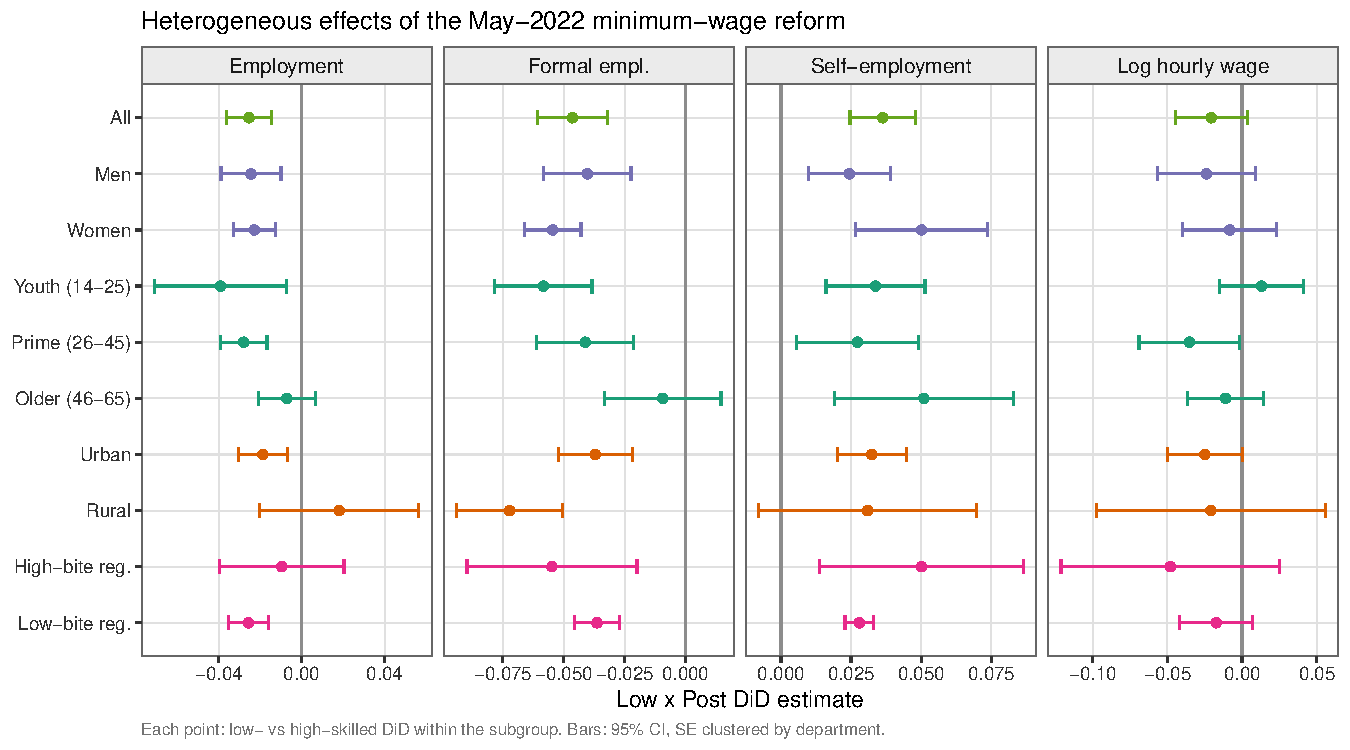
\includegraphics[width=0.98\textwidth]{fig6_heterogeneity.pdf}
\caption{Heterogeneous effects of the 2022 reform. Each point is the
$\mathrm{Low}\times\mathrm{Post}$ DiD estimate within the indicated subgroup, with
ninety-five percent confidence intervals based on standard errors clustered by department.}
\label{fig:het}
\end{figure}

\subsection{Adjustment margins}

Where exactly does the reallocation happen? Four mechanism-oriented margins sharpen
the picture (Appendix Table~\ref{tab:margins}). First, the share of low-education
wage earners employed \emph{without a written contract} rises by 3.1 percentage
points relative to high-education wage earners, so informalization operates within
wage employment and not only through exits into self-employment.\footnote{The
contract item was dropped from the reduced questionnaire applied in fifteen regions
in February 2021; I code those observations as missing rather than as lacking a
contract, which matters for this margin.} Second, employment
recomposes toward \emph{micro units}: the probability that a low-education worker is
employed in an establishment of at most twenty workers rises by 2.8 points, and small
units are precisely where enforcement is thinnest. Third, using INEI's decomposition
of informal employment (available through 2023), the displaced margin lands in the
\emph{informal sector} proper (+2.4 points) rather than in unregistered jobs inside
formal firms (+0.8, insignificant): workers did not stay with formal employers under
the table; they moved to informal productive units. Fourth, the share of wage
earners with under a year of tenure does not move, so the adjustment is not visible
as a hiring freeze among those who remain wage earners.

Two further subgroup splits locate the burden. The compositional effects are
concentrated almost entirely among \emph{non-heads} of household (secondary
earners, whose formality falls 6.8 points against a null for household heads) and
among non-indigenous workers, consistent with the urban coastal labor markets where
formal employment at the floor is concentrated. The marginal formal jobs that
dissolved were, in short, those of secondary earners in small urban firms.

\subsection{Distributional wage effects}

The absence of an average wage effect could in principle conceal offsetting movements at
different points of the wage distribution, since a minimum wage is expected to compress the
lower tail. To examine this I estimate unconditional quantile (recentered influence
function) regressions in the manner of \citet{firpo_fortin_lemieux_2009}, applying the DiD
specification to the influence function of each decile of the log real hourly wage.
Figure~\ref{fig:rif} plots the $\mathrm{Low}\times\mathrm{Post}$ coefficient across
deciles. The estimates are non-positive at every decile, mostly between $-2$ and $-4$
percent and significant at a few middle deciles; crucially, there is no positive effect at
the lower deciles, where a binding and enforced minimum wage would compress the
distribution from below. The distributional evidence therefore reinforces the absence of
a pay response: the reform did not lift the lower tail of the low-skilled wage
distribution relative to the high-skilled. This is consistent with the earnings
distribution in Figure~\ref{fig:dist}, which shows little movement toward the new floor,
and with the interpretation that in a labor market with widespread non-compliance the
statutory minimum did not bind for most low-skilled workers.

\begin{figure}[!t]
\centering
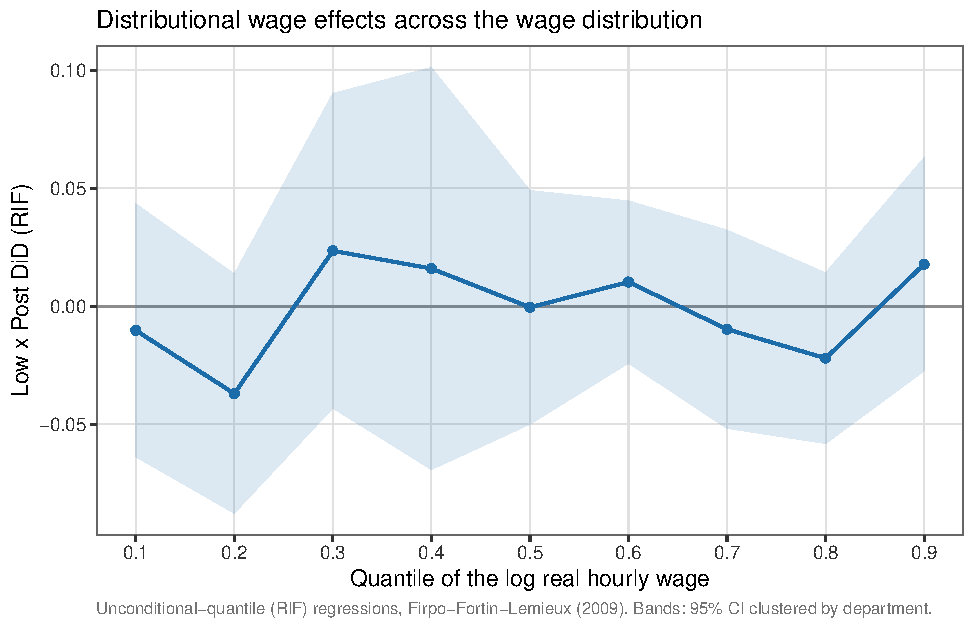
\includegraphics[width=0.72\textwidth]{fig8_rif_quantile.pdf}
\caption{Distributional wage effects. Each point is the $\mathrm{Low}\times\mathrm{Post}$
DiD coefficient from an unconditional-quantile (RIF) regression at the indicated decile of
the log real hourly wage \citep{firpo_fortin_lemieux_2009}. Bands are ninety-five percent
confidence intervals clustered by department.}
\label{fig:rif}
\end{figure}

\section{Discussion}\label{sec:discussion}

\subsection{Mechanisms}

The evidence describes a minimum wage that moved workers rather than wages. The reallocation is my most robust result: formality falls and self-employment rises, the shifts scale with the regional bite of the floor, and they are confirmed by a continuous-exposure design under randomization inference. The natural mechanism is the classic one, a binding floor in the covered sector inducing reallocation to the uncovered sector, the displacement channel that \citet{jaramillo_lopez_2006} documents for Peru and \citet{ham_2018_honduras} for Honduras. Its incidence is exactly where that mechanism predicts: among the young, among women, and in high-bite departments, the workers and places where the new floor cut deepest into the wage distribution. The panel transitions of Section~\ref{sec:transitions} identify the flow behind the stock change and refine the mechanism in one important way: retention of incumbent formal workers did not fall, while entry into formal jobs from informality dropped by nearly half, so the reallocation operated through the creation of formal matches rather than through their destruction. The floor did not push incumbents out; it closed the door on new formal matches for low-educated workers. This is the same hiring-margin adjustment that \citet{dustmann_2022} document for Germany, and it explains why the burden falls on marginal entrants, secondary earners, the young, and women, rather than on protected incumbents. The accompanying rise in hours is consistent with movement toward self-employment, where hours are less constrained. One nuance qualifies the destination of the displaced margin: in the regional design the unconditional self-employment rate does not rise with exposure (Appendix Table~\ref{tab:uncond}), so across departments the robust absolute margin is the destruction of formal employment, and the rise in the self-employment share of employment partly reflects the shrinking employment base; the absolute shift into own-account work appears in the education contrast, where the displaced workers and their closest substitutes are compared directly.

Why did no aggregate pay response accompany the reallocation? Not because the floor is a dead letter: the first-stage evidence shows that within the formal sector the spike at the old minimum migrated almost completely to the new one, so covered employers complied. The explanation is the arithmetic of coverage in a two-sector labor market \citep{ulyssea_2018}. Only 13 percent of employed low-skilled workers are formal, so even full compliance inside the formal segment moves the group's average wage very little; meanwhile pay in the informal segment drifted \emph{further} below the floor, and the two responses cancel in the aggregate. Inflation compounds this: the 2022 increase of ten percent in nominal terms met consumer price inflation of roughly eight percent, so the real value of the floor barely rose and then eroded. A floor that is honored only where labor costs are enforceable cannot lift the group's wage distribution, but it can still shape which employment arrangements firms and workers choose, and on my estimates it did. This is the same reallocation logic that \citet{dustmann_2022} document across establishments in Germany, transposed to the margin that matters in a developing economy: the boundary between formal and informal work \citep{jales_2018}.

Two caveats discipline this reading. The reallocation, while robust to specification and to design-based inference, is sensitive to modest violations of parallel trends in the education contrast \citep{rambachan_roth_2023}, and it does not reappear around the 2025 reform, where the same design and the same magnitudes yield nulls on every margin and a small opposite-signed self-employment estimate. I interpret the contrast between the two episodes as state dependence, and Section~\ref{sec:reconciliation} probes the two candidate state variables directly: the evidence favors the position of the floor in the formal pay distribution, the 2022 increase swept a band holding a quarter of low-educated formal pay while the 2025 increase swept a thinner one, and it rejects the labor-market-churn version, since formal match creation was in fact higher on the eve of 2025. The entry-margin evidence of Section~\ref{sec:transitions} identifies the margin through which any such state dependence must operate: the creation of new formal matches, whose profitability the floor governs. I cannot, however, fully exclude the alternative reading, that residual recovery dynamics correlated with education contribute to the 2022 compositional estimates; the dose-response and continuous-exposure evidence is what tilts me toward a causal interpretation, since differential recovery by education has no reason to track the pre-reform regional Kaitz index.

\subsection{Reconciliation with the previous literature}\label{sec:reconciliation}

My results sit comfortably with some of the prior evidence and in tension with the rest, and the pattern is itself informative. They echo the older Peruvian work of \citet{jaramillo_lopez_2006}, who found the 2003 reform largely innocuous with displacement toward informality, and of \citet{cespedes_2005}, who found effects concentrated among the young. They are consistent with the broad international finding that minimum wage increases in this range produce small employment effects \citep{card_krueger_1995, cengiz_2019}.

The tension is with the most recent Peruvian study. \citet{jimenez_2023} finds that the 2016 reform raised formal wages by four to five percent and increased formality, a lighthouse pattern that I do not reproduce for 2022. Three differences plausibly account for the divergence. The 2016 increase occurred in a low-inflation period, so its real bite was larger and more durable than that of the inflation-eroded 2022 increase. The identification differs: \citet{jimenez_2023} uses a department-level dose defined on the formal wage distribution, while I contrast low- and high-education workers at the individual level, a design that places more weight on the large informal segment of the low-skilled. And the macroeconomic setting differs, stable growth in 2016 against a post-pandemic recovery in 2022. One observation helps to sort out these explanations: 2016, the lighthouse episode, was itself a calm year, and so was 2025, in which I find no effects at all, so macroeconomic state alone cannot be the whole story. What separates 2016 from 2025 is the \emph{level} of the floor when the increase arrived: in 2016 the minimum stood well below the median wage and a real increase could plausibly propagate as a norm, whereas by 2025 the floor already exceeded the national median, so a further increase started from a level that practice had already ceased to honor for the marginal worker. On this reading the three episodes are ordered by two state variables, namely how high the floor already sits in the wage distribution and how much re-sorting the labor market is doing: a moderate floor rising in a stable market can lift norms (2016); a high floor rising amid post-pandemic re-sorting moves the composition margin (2022); and a high floor rising in a settled market moves nothing (2025).

Because a story with two free state variables can rationalize almost anything, I probe both directly and let the data discard one. The floor-position variable behaves as the story requires: on the eve of the 2022 reform, 24 percent of low-educated formal wage earners were paid inside the band the incoming floor was about to sweep and 16 percent bunched at the old floor, whereas on the eve of the 2025 reform those shares had fallen to 17 and 14 percent. The re-sorting variable does not: the new-hire share among low-educated formal workers was \emph{higher} in 2024 (41 percent) than before the 2022 reform (32 percent), so the 2025 null cannot be attributed to a scarcity of new formal matches. A department-level dose test points the same way: interacting the education contrast with pre-reform formal match creation yields no gradient in either episode, with or without the Kaitz control.\footnote{The state-variable moments and the dose estimates are included in the replication package (\texttt{state\_premise.csv}, \texttt{state\_dose.csv}).} I therefore retire the churn version of the argument and rest the interpretation on the floor's position: the entry margin closes when the incoming floor sweeps a dense band of formal pay, as in 2022, and has little left to close when the floor has already moved past the range that formal pay practice honors, as in 2025. The swept-band contrast is real but modest, so I present this as the reading most consistent with the evidence rather than as established.

\subsection{External validity and limitations}

Five limitations bound the interpretation. First, identification rests on the assumption that, absent the reform, low- and high-education workers would have followed parallel paths. I test this where possible and bound the consequences of its failure; the formality pre-trends are flat, but the wage pre-trend test rejects on account of a single early-2021 quarter, and the employment series carries a clear recovery pre-trend, which is why I state the wage conclusion as ``no detectable gain'' rather than a precise null and treat the employment-level result as inconclusive. Second, the design identifies effects on low-skilled workers relative to high-skilled workers. The comparison group is not entirely unexposed (40 percent of high-skilled wage earners sat below the new floor pre-reform), so the estimates are relative objects that, to first order, understate the effect on the fully exposed; the continuous-exposure design partly addresses this by dispensing with the comparison group. Third, the main design uses repeated cross-sections; the ENAHO Panel analysis of Section~\ref{sec:transitions} addresses the flow-versus-stock distinction directly, but it is annual rather than quarterly, its pre-reform benchmark includes transitions out of the pandemic year 2020, and its formal-base samples are modest, so I treat it as corroborating the mechanism rather than as delivering precise magnitudes. Fourth, informality in 2024 is measured with a reconstructed indicator rather than the official one; within the 2025 validation window the indicator is reconstructed consistently in every quarter, but the 2024 splice adds measurement error to the tail of the 2022 event study. Finally, the window spans at most ten clean post-reform quarters, so I speak to short- and medium-run effects and not to the long-run adjustment of capital or firm entry and exit.

\subsection{Policy implications}

The results carry a sober message for minimum wage policy in a high-informality economy. A floor that goes unenforced for most of its intended beneficiaries does little to raise their pay, and where it does bind, in the formal sector, it may nudge some workers toward less protected arrangements. Raising the minimum wage is therefore an imperfect instrument for lifting the earnings of the low-skilled in Peru, a conclusion that echoes \citet{jaramillo_lopez_2006}. This is not to say the minimum wage is harmless or useless; my estimates are relative and my window is short. But it does imply that formalization and enforcement are preconditions for the floor to reach the workers it is designed to protect. Absent them, the margin of adjustment is the composition of employment rather than the level of pay.

\section{Conclusion}\label{sec:conclusion}

I have studied how Peru's 2022 minimum wage increase, from 930 to 1,025 soles, affected
workers with different levels of education, using quarterly ENAHO data and a
difference-in-differences design that exploits the sharply different exposure of low- and
high-education workers to a single national reform. My central finding is that the reform
shifted the composition of low-skilled employment rather than the level of low-skilled
pay: formal employment fell by 4.6 percentage points, a fifth of its baseline, and
self-employment rose by 3.6 points, with formality pre-trends that pass their joint
test and a residual drift that I quantify and adjust for, larger shifts where the floor
cut deeper into the regional wage distribution, and confirmation from a
continuous-exposure design under randomization inference. Linked panel data locate
the margin: incumbent formal workers were retained, while entry into formal jobs by
low-educated workers fell by nearly half, so the floor operated by closing the door
on new formal matches rather than by dissolving existing ones. No pay response accompanied the
shift: relative wages of low-education workers did not rise at the mean or anywhere in
the distribution, and the share of wage earners paid below the floor did not fall,
pointing to non-compliance as the reason the floor could not lift pay. The overall
employment effect cannot be pinned down and is confounded by the uneven post-pandemic
recovery. Around the identically sized reform of January 2025, neither wages nor
composition responded. Probing the contrast directly favors a floor-position reading
over a labor-market-churn one: the 2022 increase swept a band holding a quarter of
low-educated formal pay, while the 2025 increase swept a thinner band in a
distribution the floor had already outrun, even though formal match creation was, if
anything, higher in 2024. The reallocation margin operates when the incoming floor
cuts through the range where formal pay actually sits, and lies dormant when it has
moved past it.

The most economical reading of these results is that, in a labor market where informality
is pervasive and enforcement is weak, a moderate and inflation-eroded increase in the
statutory minimum does not lift the pay of the low-skilled; what it moves, when it moves
anything, is the allocation of workers between formal and informal arrangements. This
qualifies the lighthouse view of the Peruvian minimum wage that emerges from studies of
earlier reforms and points to the informal margin as the central channel of adjustment.

Two directions for future research follow. The first is to sharpen the transition
evidence with higher-frequency linked data, either the monthly EPEN or administrative
payroll records from the Planilla Electrónica, which would time the hiring-margin
response within the year and follow the same firms and workers across both reforms;
my annual panel establishes the margin but not its fine dynamics. The second is to
study the interaction between minimum wage policy and enforcement directly, since my
results suggest that the returns to raising the floor depend on whether the floor can be
made to bind. As additional post-reform quarters accumulate, it will also become possible
to trace the longer-run adjustment that a short window such as mine cannot capture.


\newpage
\bibliography{paper/references}

\newpage
\appendix
\section{Data appendix}\label{app:data}

\subsection{Sample and variable construction}

I pool the twenty quarterly ENAHO employment modules (module 500) for 2021Q1--2025Q4;
the main analysis uses 2021Q1--2024Q4 and the validation uses 2024Q1--2025Q4. The
working-age sample comprises individuals aged 14 to 65 with non-missing education. All
statistics use the module employment weight (\texttt{fac500a}). This weight is
calibrated so that the full year of interviews expands to the annual population
projection; each quarterly subsample therefore expands to roughly one fourth of the
population, which is immaterial for the weighted means, shares, and regression
estimates used throughout (numerator and denominator scale together) and would matter
only for population totals, which I never estimate. The quarterly partition follows
the interview month and matches the survey's own design: quarterly national inference
is an official inference level of ENAHO in the technical sheets of both 2021 and 2025,
and the non-panel sample revisits the same conglomerates in the same months every
year. I verify both properties in the microdata for the full window: all 5{,}359
conglomerates appear in every year from 2021 to 2025, the overlap of primary sampling
units between the same quarter of consecutive years ranges from 70 to 92 percent
(against 2 to 5 percent between different quarters), and each quarter is an
internally balanced replica of the design. Two survey changes over the window are
worth recording. First, the mixed interview modality adopted during the pandemic
(face-to-face prioritized, telephone follow-up for absent members) remained the
standard through 2025, so the mode is broadly consistent across my study period; the
one exception is February 2021, when a reduced telephone questionnaire in fifteen
regions dropped, among other items, the contract-type question (missing for half of
that month's wage earners), which affects none of the baseline outcomes (2021
informality comes from INEI's official indicator and income items were retained) and
is handled explicitly in the one appendix margin that uses contracts. Second, the
2025 technical sheet describes the design as two-stage with urban conglomerates of
about 140 dwellings, against the multi-stage description of 2021; the conglomerate
identifiers and counts are nonetheless continuous across the window, so this is a
reframing of the documentation rather than a break in the sample. Departments are the 25
first-level administrative units derived from the first two digits of \texttt{ubigeo};
the urban indicator is derived from the sampling stratum.

\paragraph{Education and skill groups.} Educational attainment is ENAHO variable
\texttt{p301a}. I verified its coding against the weighted attainment distribution.
Low-skilled workers are those with \texttt{p301a} in 1--6 (no education through complete
secondary); high-skilled workers are those with \texttt{p301a} in 7--11 (non-university
higher through postgraduate). Special education (code 12) and missing values are excluded.

\paragraph{Labor income and wages.} ENAHO records the pay of wage earners per pay period:
\texttt{p524a1} is the gross payment including overtime and \texttt{p523} its frequency
(daily, weekly, fortnightly, or monthly). Fifty-four percent of low-education wage
earners are paid at non-monthly frequencies, against fifteen percent of high-education
wage earners, so I convert all payments to monthly equivalents using the same factors
implied by INEI's own annualized income variable (\texttt{i524a1}): 25 for daily, $52/12$
for weekly, 2 for fortnightly, and 1 for monthly. The full weighted frequency
distribution among private wage earners with valid earnings is 2 percent daily, 45
weekly, 9 fortnightly, and 45 monthly for the low-education group, against 1, 18, 6,
and 76 percent for the high-education group; the frequency variable is never missing
in that sample. Wage earners comprise employees and
domestic workers (\texttt{p507} in $\{3,4,6\}$); domestic workers have been entitled to
the minimum wage since Law 31047. For employers and own-account workers, labor income is
net profit (\texttt{p530a}), which is already monthly. Because reported income refers to
the month before the interview, I deflate at that reference month (January interviews
roll back to December of the previous year) using the Lima consumer price index
rebased to December 2021, and I evaluate the statutory minimum in force in the same
reference month when classifying workers as paid below the floor. The real hourly wage
divides monthly-equivalent labor income by $4.345$ times weekly hours in the main
occupation (\texttt{p513t}; INEI's imputed hours variable \texttt{i513t} substitutes
where \texttt{p513t} is missing, but no observation in the wage-analysis sample and
fewer than 0.01 percent of the hours sample require it). Wage outcomes exclude public-sector
workers, whose pay is set by separate scales, and are winsorized once at the 0.5th and
99.5th percentiles of the pooled private wage-earner sample.

\paragraph{Informality.} INEI's official informal-employment indicator (\texttt{ocupinf},
coded 1 for informal and 2 for formal in these files) is present for 2021--2023 but absent
for 2024--2025. I reconstruct a consistent indicator from primitives available in every
year. A wage employee or domestic worker is classified as formal if affiliated to a
pension system (\texttt{p558a1}--\texttt{p558a4}, whose selected options are marked with
their option codes rather than with ones) or holding a formal labor contract
(\texttt{p511a} in 1--6); an employer or own-account worker is classified as formal if the
productive unit is registered (\texttt{p510a1}); unpaid family workers are always informal.
Validated against \texttt{ocupinf} on the overlapping years 2021--2023, this rule agrees
with the official classification for 87.8 percent of employed workers and yields an
informality rate of 74.9 percent against the official 79.1 percent. I use the official
indicator wherever available and the reconstruction only for 2024--2025; within the
2024--2025 validation window the indicator is reconstructed in every quarter, so it is
measured consistently there.

\paragraph{Minimum wage and bite.} The statutory minimum wage schedule is taken from the
decrees and verified against the Banco Central de Reserva del Perú series (PN02124PM);
the CPI deflator is BCRP series PN38705PM (Lima, December 2021 $=$ 100), and both inputs
are regenerated by a documented script in the replication package. The department Kaitz
index is the ratio of the post-reform minimum (1,025 soles) to the department's
pre-reform (2021Q1--2022Q1) weighted median monthly-equivalent wage of private wage
earners. The fraction-affected measure is the pre-reform weighted share of private wage
earners paid below 1,025 soles.

\paragraph{The ENAHO Panel.} The transition analysis of Section~\ref{sec:transitions}
uses the ENAHO Panel 2020--2024 (INEI survey 978, published November 2025), whose
employment module (\texttt{enaho01a-2020-2024-500-panel.dta}) contains one record per
person with year-suffixed variables for 2020 through 2024. Persons observed in both
years of a pair are flagged by the indicators \texttt{perpanel} (23,983 linked persons
for 2021--22 and 23,245 for 2022--23) and weighted with the INEI panel expansion
factors \texttt{facpanel}, which adjust for attrition and non-response; official
inference for consecutive-year pairs is national, urban and rural, and by natural
region. Employment states replicate the cross-section definitions exactly: employed
is \texttt{ocu500}${}=1$; the formal private state requires private-sector employment
with a formal job; informality uses the official \texttt{ocupinf} where released and
the Rule-F reconstruction above elsewhere; self-employment comprises own-account
workers and employers. Base-year education defines the skill groups. Because the
panel is annual and the reform took effect on 1 May 2022, pair-observations are
classified with the 2022 interview month as described in the notes to
Table~\ref{tab:transitions}.

\paragraph{Protest intensity.} The department-level intensity of the 2022--23
political crisis is measured from the monthly conflict reports of the Presidencia del
Consejo de Ministros (Secretar\'ia de Gesti\'on Social y Di\'alogo, ``Reporte de
Conflictos Sociales''), whose crisis-monitoring tables record the maximum number of
persons mobilized in protest actions in each department in each week and month. I take
each department's maximum across the January and February 2023 reports, the two months
in which national mobilization peaked (the December-2022 report predates the table),
divide it by the department's working-age population (four times the mean quarterly sum
of the ENAHO expansion weights), and standardize the result across the 25 departments.
The transcribed table and the source documents are included in the replication
package.

\subsection{Supplementary results}

Table~\ref{tab:ddd} reports the triple-difference estimates and Table~\ref{tab:loo}
the leave-one-out stability ranges discussed in Section~\ref{sec:robustness};
Tables~\ref{tab:expocells}--\ref{tab:margins} collect the exposure-design diagnostics,
the sectoral and occupational checks, the selection bounds and power calculations, the
synthetic-DiD and pre-test-power results, and the adjustment margins.
Table~\ref{tab:crisis} reports the political-crisis robustness of the continuous
regional-exposure design and Table~\ref{tab:uncond} the unconditional compositional
outcomes, both discussed in Section~\ref{sec:robustness}.
Table~\ref{tab:placebo} reports the in-time placebo reforms and confirms that the wage
placebos are null while the employment placebos are contaminated by the pandemic
pre-trend. The doubly robust estimates of \citet{santanna_zhao_2020} appear alongside
the two-way fixed-effects estimates in Table~\ref{tab:main}.
Figure~\ref{fig:val2025} shows the event study around the January-2025 reform used in
the out-of-sample validation.

\input{../../tables/tab_triplediff}

\input{../../tables/tab_leaveoneout}

\input{../../tables/tab_exposure}

\input{../../tables/tab_sector_occ}

\input{../../tables/tab_lee_mde}

\input{../../tables/tab_sdid_power}

\input{../../tables/tab_margins}

\input{../../tables/tab_migration}

\input{../../tables/tab_crisis}

\input{../../tables/tab_uncond}

\paragraph{Deflators.} All wage regressions include quarter fixed effects, which
absorb national inflation, so log-wage DiD estimates are invariant to the national
deflator; and the bite measures compare nominal wages with the nominal statutory
floor, so they involve no deflation at all. Department-specific price deflation would
matter only for cross-departmental comparisons of real wage \emph{levels}, which play
no role in the identification.

\begin{figure}[!t]
\centering
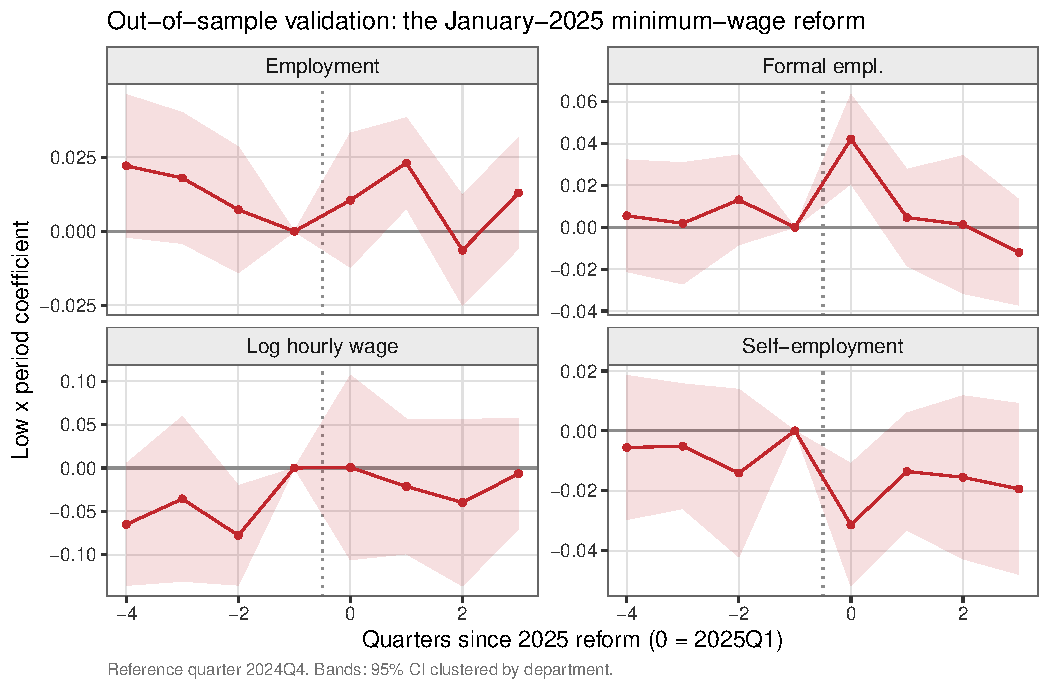
\includegraphics[width=0.9\textwidth]{fig9_validation2025.pdf}
\caption{Event study around the January-2025 reform (out-of-sample validation). Coefficients
on the interaction of the low-skill indicator with quarter indicators, reference quarter
2024Q4. Bands are ninety-five percent confidence intervals clustered by department.}
\label{fig:val2025}
\end{figure}

\begin{table}[!tbp]\centering
\caption{In-time placebo reforms (pre-reform window only)}\label{tab:placebo}
\begin{threeparttable}
\input{../../tables/tab_placebo_body}
\begin{tablenotes}\footnotesize
\item Notes: Each entry is the $\mathrm{Low}\times\mathrm{Post}$ coefficient from a placebo
DiD that assigns a fake reform to the indicated quarter, estimated using only pre-reform
data (2021Q1--2022Q1). Standard errors clustered by department in parentheses; all estimates
are weighted by ENAHO survey weights. $^{*}p<0.1$, $^{**}p<0.05$, $^{***}p<0.01$.
\end{tablenotes}
\end{threeparttable}
\end{table}


\end{document}
